\chapter{Lösung der Aufgabenstellung}

In diesem Kapitel wird das Vorgehen zur Entwicklung eines DML-Flachlautsprechers beschrieben. Dabei wird zuerst die verwendete Hard- und Software tabellarisch aufgelistet, um die in dieser Arbeit gegebenen Rahmenbedingungen zu erläutern. Anschließend werden die wichtigsten Hardwarekomponenten, welche den Exciter, die DML-Platte sowie die verwendete Stereoanlage mit Equalizer umfassen, einzeln beschrieben. Da deren Eigenschaften ausschlaggebend für die akustischen Eigenschaften des DML sind. Anhand der technischen Eigenschaften der Audiogeräte wird ein Konzeptentwurf hinsichtlich der Umsetzbarkeit und Eignung für das vorliegende Entwicklungsvorhaben diskutiert. Dabei wird aufgezeigt, welches der gegebenen Plattenmaterialien für den Bau der DML-Flachlautsprecher verwendet wird und welche Panelabmessungen sinnvoll sind. Anschließend wird sich für eine Umsetzung unter Berücksichtigung der Materialparameter entschieden.
Auf dem Konzept aufbauend wird eine Simulation aufgesetzt, welche zur Bestimmung der idealen Anregerposition für die gegebenen Parameter führen soll. Anhand der in der Simulation berechneten Ergebnisse werden diese Positionen im realen Versuchsaufbau vermessen. Die Ergebnisse werden anschließend diskutiert und verglichen.


\section{Verwendete Hardware}

Die in dieser Arbeit verwendete Software für die Simulation der Platten sowie für den Versuchsaufbau wird mit der verwendeten Hardware, welche zum Bau der DML und zur Vermessung der Lautsprecher verwendet werden, in der folgenden Tabelle 3.1 aufgelistet.

\begin{table}[h]
\centering
\caption{Verwendete Hard- und Software}
\label{tab:hardware}
\begin{tabular}{|p{3,5cm}|p{3cm}|p{3,5cm}|}
\hline
\textbf{Hersteller} & \textbf{Modell} & \textbf{Beschreibung} \\
\hline
 Dayton Audio & DAEX32EP-4 & Körperschallwandler \\
 \hline
 Wangine Electronics Co. & WPA-600 PRO & Leistungsendstufe \\
 \hline
 Wangine Electronics Co. & WVQ-600 PRO & Vorverstärker \\
 \hline
 3A Composites GmbH & KAPA Line & Sandwichplatte 15 mm \\
 \hline
 3A Composites GmbH & KAPA Graph & Sandwichplatte 5 mm \\
 \hline
 National Instruments & LabVIEW 2013 & Messsoftware \\
 \hline
 National Instruments & NI PXI-1033 & Chassis \\
 \hline
 National Instruments & NI PXI-4472B & Datenerfassungskarte \\
 \hline
 National Instruments & NI PXI-6733 & Datenausgabekarte \\
 \hline
 National Instruments & NI SCC-68 & Anschlussblock \\
 \hline
 Sinuslive & HL-406 & High-Low Adapter \\
 \hline
 iSEMcon & EMM-13D082S & Messmikrofon \\
 \hline
 COMSOL Inc. & COMSOL Multiphysics 6.4 & Simulationssoftware \\
\hline
\end{tabular}
\end{table}

\clearpage


\subsection{Der Exciter}

Zum Anregen der Platte werden Körperschallwandler der Firma Dayton Audio verwendet. Die Abbildung \ref{fig:Exciter} zeigt die Vorder- und Rückseite des verwendeten Exciters, an der Rückseite des Exciters ist die Kontaktfläche, welche mit einem doppelseitigen Klebeband von 3M versehen ist.


\begin{figure}[H]
	\centering
	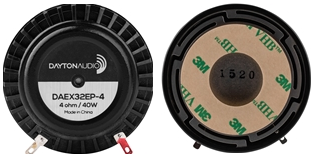
\includegraphics[width=0.6\textwidth]{pictures/Exciter.png}
	\caption{Dayton Audio Exciter \cite{DaytonAudio2024}}
	\label{fig:Exciter}
\end{figure}

Das Modell ist der Typ DAEX32EP-4, welcher mit einer Leistung von 40 W RMS bei einer Impedanz von 4 $\Omega$ zu den leistungsstärkeren Modellen seiner Klasse zählt \cite{DaytonAudio2024}. Dieser Exciter wird mithilfe einer Klebefläche, welche einen Innendurchmesser von 21,75 mm und einen Außendurchmesser von 41,75 mm hat, an die vorgesehene Platte geklebt. Damit wird eine schlüssige Kraftübertragung von Exciter auf Platte gewährleistet. Der Frequenzverlauf des Exciters wurde vom Hersteller vermessen, dabei wurde eine ungefähr 30 cm x 30 cm und 1,3 cm starke Sandwichplatte mit Schaumkern mit einem außermittig platziertem Exciter in einem Freifeldraum angeregt. Der SPL-Verlauf über der Frequenz ist dabei relativ linear im Bereich 70 bis 5.000 Hz bei einem SPL von ca. 83 dB, ab 5.000 bis 20.000 Hz fällt der SPL auf ca. 68 dB ab.
Der SPL über Frequenz Graph und alle weiteren zugehörigen technischen Daten sind dem Datenblatt in Anhang A zu entnehmen.

\clearpage

\subsection{Plattenmaterial}

Als DML-Material wurden zwei Platten in Sandwichbauweise der Firma 3A Composites zur Verfügung gestellt. Die beiden Platten haben eine Größe von \SI{1}{\meter} x \SI{0,7}{\meter} und unterscheiden sich im Wesentlichen in ihrer Stärke und dem Trägermaterial.
Die KAPA Line Platte hat eine Stärke von \SI{15}{\milli\meter}, dabei besteht die Deckschicht aus einer Faltschachtelkartonschicht, welche mit handelsüblichen Klebern und Farben bearbeitet werden kann. Demzufolge sollten die Exciter problemlos an der Deckschicht verklebt werden können. Der Kern der Sandwichplatte besteht aus Polyurethan-Hartschaum (kurz PUR).
Die KAPA Graph Platte hat eine Stärke von \SI{5}{\milli\meter} mit einer Deckschicht aus einem hochwertigen pH-neutralen Zellstoffkarton und hat wie KAPA Line gute Bearbeitungseigenschaften. Beide Sandwichplatten haben einen PUR-Hartschaumkern, welcher gegen eine Vielzahl von Klebern und Lösungsmitteln beständig ist und sich mit einem Cuttermesser gut bearbeiten lässt.
 

\begin{figure}[H]
	\centering
	\includegraphics[width=0.6\textwidth]{pictures/KAPA_Vergleich.png}
	\caption{Vergleich KAPA Graph \& KAPA Line}
	\label{fig:KAPA_Vergleich}
\end{figure}

In der Abbildung \ref{fig:KAPA_Vergleich} sind die beiden KAPA Sandwichplatten dargestellt. Gut zu erkennen ist der Stärkenunterschied, welcher mittels Schublehre gut ablesbar gezeigt wird, sowie der Sandwich-Kern, welcher bei beiden Platten aus PUR-Hartschaum besteht. Nicht gut zu erkennen ist die Deckschicht, welche bei beiden Platten \SI{0,5}{\milli\meter} stark ist und den Schaumkern auf der oberen und unteren Seite vollständig bedeckt.
Im Wesentlichen unterscheiden sich die Platten in ihrem E-Modul und der daraus resultierenden Steifigkeit sowie der Dichte und dem daraus resultierenden Gewicht. 


\subsection{Verstärker und Equalizer}

Bei der eingesetzten Stereoanlage handelt es sich um die WPA-600 Pro Leistungsendstufe der Firma Wangine Electronics Co., welche als Verstärker zur Ansteuerung der verwendeten Körperschallwandler dient.

\begin{figure}[H]
	\centering
	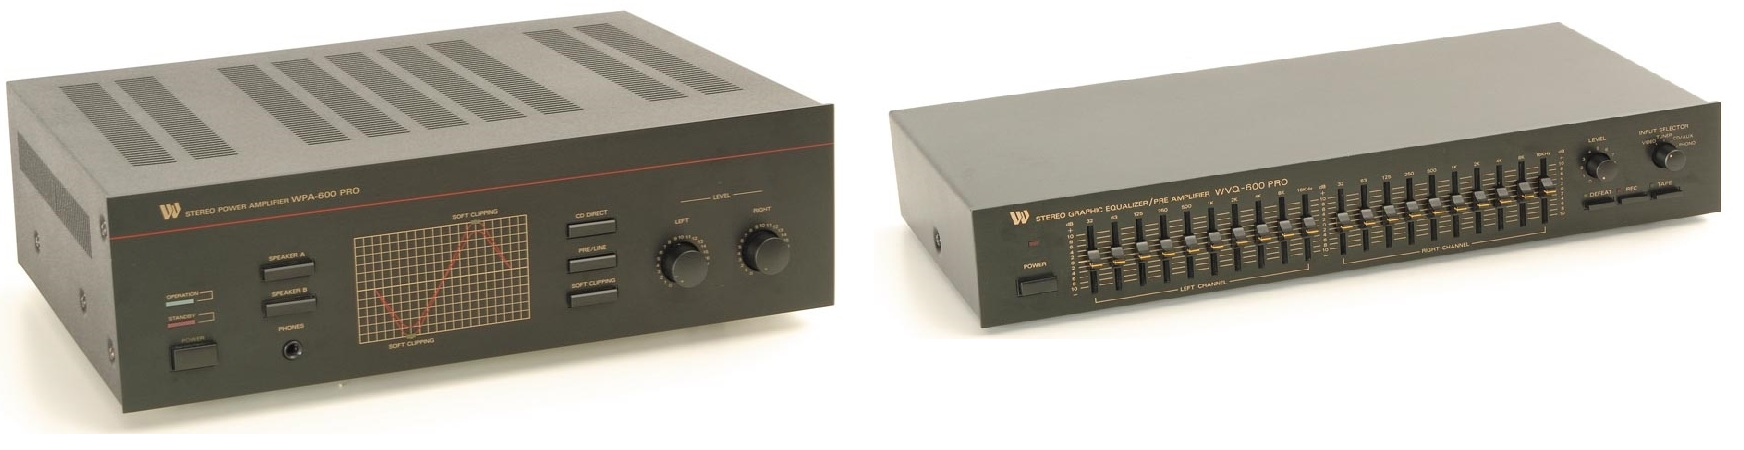
\includegraphics[width=0.6\textwidth]{pictures/Stereo_EQ.png}
	\caption{WPA-600 Pro Leistungsendstufe \& WVQ-600 Pro Equalizer \cite{Wangine2024}}
	\label{fig:Stereo_EQ}
\end{figure}

Dabei stellt sie eine ausreichende elektrische Leistung für unterschiedliche Lautsprecherimpedanzen im Bereich von 4 $\Omega$ bis 16 $\Omega$ bereit. Die Endstufe arbeitet im Stereobetrieb und zeichnet sich durch einen breiten Frequenzgang sowie einen geringen Klirrfaktor aus, wodurch eine weitgehend verfälschungsfreie Signalverstärkung gewährleistet wird. Die zugehörigen technischen Kenndaten sind dem Datenblatt im Anhang B zu entnehmen. 
Die Endstufe kann in Kombination mit dem passenden Vorverstärker WVQ-600 Pro desselben Herstellers betrieben werden. Der WVQ-600 Pro kann das Eingangssignal verstärken und verfügt über einen integrierten grafischen Equalizer, welcher 10 Frequenzbänder pro Kanal um jeweils ±10 dB anpassen kann. Dadurch lässt sich der Klang gezielt an die akustischen Eigenschaften des DML-Systems anpassen. Die Kombination aus Stereoanlage und Equalizer wird sowohl im Versuchsaufbau als auch im späteren Gebrauch verwendet. 

\clearpage

\section{Konzeptentwicklung des DML-Flachlautsprechers}

Bei der Konzeptentwicklung des DML-Flachlautsprechers werden verschiedene Umsetzungsmöglichkeiten dargestellt und anhand ihrer technischen Realisierbarkeit, akustischen Performance sowie ihrer wirtschaftlichen Umsetzbarkeit untersucht, diskutiert und bewertet. Anschließend wird sich für ein Konzept entschieden, welches simuliert und vermessen wird. Neben der grundsätzlichen Systemauslegung wird auch die spätere Lagerung beziehungsweise Aufhängung der Platte betrachtet, da diese das Schwingungsverhalten und somit die akustische Performance maßgeblich beeinflussen kann \cite{Bai2001}.

Die Entscheidungsfindung basiert auf einer gewichteten Nutzwertanalyse, die sowohl technische Kriterien als auch die spezifischen Rahmenbedingungen aus Kapitel 3.1 berücksichtigt. Dadurch wird eine transparente und nachvollziehbare Auswahl des geeigneten Systemkonzepts gewährleistet.

Die Entwicklung eines DML-Flachlautsprechers erfordert grundlegende Entscheidungen bezüglich folgender zentraler Systemparameter:

\begin{enumerate}
    \item Frequenzweichenkonfiguration
    \item Plattenkonfiguration
    \item Plattenlagerung
    \item allgemeine Systemauslegung. 
\end{enumerate}

Diese werden in den folgenden Unterkapiteln erläutert und bestimmt.

\subsection{Frequenzweichenkonfiguration}

Die Frequenzweichenkonfiguration befasst sich mit der möglichen Verwendung von Frequenzweichen und dem Bau eines Zwei- oder Drei-Wege-Systems, welches mehrere Platten oder eine mögliche Subwoofereinbindung im System in Betracht zieht. Dabei kann zwischen einer passiven Frequenzweiche, welche aus Spulen, Kondensatoren und Widerständen besteht, und einem digitalen Signalprozessor-Weiche, kurz DSP-Weiche, unterschieden werden.
Während passive Weichen das Signal nach dem Verstärker in die verschiedenen Frequenzbereiche trennt, ermöglicht ein DSP die digitale Signalverarbeitung in Echtzeit. Ein DSP kann neben der Frequenztrennung auch als Equalizer verwendet werden, was insbesondere bei DML-Systemen von Vorteil sein kann. 
Es ist zu beachten, dass im Übergangsbereich der Frequenzweichen komplexe Interferenzmuster entstehen können, die zu räumlich variierenden Übertragungsfunktionen führen können \cite{Moeser2005}.

Ein DML 2-Wege-System mit Subwoofer-Integration umfasst einen DML-Flachlautsprecher, welcher den Mittel- und Hochtonbereich abdeckt, und einen Subwoofer, welcher den Tieftonbereich wiedergibt. Dabei wird das Frequenzband in einen Tieftonbereich, typischerweise bis etwa 100 Hz, und einen Mittel- bis Hochtonbereich oberhalb dieser Trennfrequenz aufgeteilt. Ein Vorteil dieser Konfiguration besteht darin, dass die Trennfrequenz unterhalb des sensiblen Vokalbereichs liegt und die Sprachverständlichkeit somit nicht beeinträchtigt wird \cite{Weinzierl2025}. Sollte die Trennfrequenz unterhalb des Vokalbereichs liegen, ist eine Subwoofereinbindung denkbar.

Ein 3-Wege-System unterteilt den Frequenzbereich in ein Tief-, Mittel- und Hochtonspektrum. Bei dieser Bauweise werden separate Treiber für Tief-, Mittel- und Hochtonbereich eingesetzt. Diese Bauweise wird im Zusammenhang mit DML-Flachlautsprechern kritisch bewertet, da die Frequenztrennungen im Stimmbereich zu Verständlichkeitsproblemen und Phasenverschiebungen führen können, die selbst durch digitale Signalverarbeitung nur schwer vollständig korrigierbar sind. Typische Trennfrequenzen von 3-Wege-Systemen liegen im Bereich von etwa 500 bis 1.000 Hz für den Übergang zwischen Tief- und Mittel-ton sowie zwischen 4.000 und 5.000 Hz für den Übergang zwischen Mittel- und Hochtonbereich \cite{Weinzierl2025}. Damit befindet sich mindestens eine Trennfrequenz im sensiblen Vokalbereich, weshalb eine 3-Wege-Bauweise für ein DML-System nicht berücksichtigt wird.

Das Fullrange-System ohne Frequenzweiche stellt die einfachste Umsetzung eines DML-Flachlautsprechers dar. In diesem Fall deckt das Panel den gesamten hörbaren Frequenzbereich ab, wobei das elektrische Audiosignal ungefiltert dem Lautsprecher zugeführt wird. Dadurch entfallen phasenbedingte Verzerrungen, wie sie durch Frequenzweichen entstehen können \cite{Moeser2005}. Anhand der Einfachheit dieses Aufbaus, welche zugleich eine unverzerrte Wiedergabe über die Lautsprecher verspricht, wird dieser Aufbau favorisiert. 


\subsection{Materialkonfiguration}

Mit der Materialkonfiguration ist die Auswahl zwischen den beiden gegebenen KAPA Sandwichplatten anhand ihrer mechanischen Eigenschaften sowie die Bestimmung der Größe gemeint. Dabei spielt die Steifigkeit eine tragende Rolle. Die Biegesteifigkeit wird in den Datenblättern der Sandwichplatten Anhang C und D, nicht angegeben. Daher wird die Biegesteifigkeit näherungsweise mit der Gleichung \ref{eq:biegesteifigkeit} bestimmt. 
Dabei beträgt die Dicke der Deckschicht \SI{0,5}{\milli\meter} pro Seite, also \SI{1}{\milli\meter} insgesamt. Das E-Modul wird aus dem Datenblatt von KAPA Graph entnommen. 
Da das E-Modul für KAPA Line nicht im Datenblatt vorhanden ist, beide Platten aber dieselbe Schaumschicht und eine ähnliche Stützstruktur haben, wird für beide das E-Modul von KAPA Graph verwendet. Daraus ergibt sich für die beiden Materialien: 

Daraus ergeben sich die folgenden Biegesteifigkeiten:

\begin{equation}
B_{\text{graph}} \approx 12{,}8 \, \text{N} \cdot \text{mm}^2
\end{equation}

\begin{equation}
B_{\text{line}} \approx 156{,}8 \, \text{N} \cdot \text{mm}^2
\end{equation}

Es ist zu erkennen, dass die ausgerechnete Biegesteifigkeit der Sandwichplatten von KAPA Line wesentlich größer ist als von KAPA Graph. Das liegt vor allem an der dreimal höheren Plattenstärke der KAPA Line Platte im Gegensatz zu der KAPA Graph Platte. Unter Berücksichtigung der Biegesteifigkeit und den zugehörigen Flächenmasse, welche aus den Datenblättern entnommen wurden, bietet sich die Sandwichplatte aus KAPA Line besser als DML-Panel an als aus KAPA Graph. Diese Annahme ist alleinig auf die Materialparameter im Vergleich zurückzuführen, da KAPA Line im Vergleich eine mehr als zehnmal so große Biegesteifigkeit aufweist bei einem Flächengewicht, welches gerade einmal 1,45 mal so groß ist wie KAPA Graph.

Nach der Materialauswahl müssen nun die Abmaße der Platte bestimmt werden. Die Größe der Platte ist ausschlaggebend für die angeregten Moden und daraus entstehenden Frequenzen. Da der DML in dieser Arbeit als Fullrange-System konzipiert wird, muss die Größe so gewählt werden, dass sowohl im Tiefton als auch im Mitten- und Hochtonbereich eine gute Wiedergabe gegeben ist. Zudem soll die Plattenfront als Informations- und Werbefläche verwendet werden. 
Dafür werden Plakate in DIN-Größe, welche ein Seitenverhältnis von 1:1,414 haben, auf die Vorderseite der Platte geklebt. Aufgrund dessen ist von einer quadratischen Auslegung abzusehen. Aus diesen Gründen wird die Plattengröße anhand eines Seitenverhältnisses 1:1,618, in der Mathematik bekannt als Goldener Schnitt $\varphi$, verwendet. 

Dieser Goldene Schnitt wird vor allem in der DML-DIY-Community empfohlen und ist für gute akustische Eigenschaften bekannt. Aus mathematischer Sicht betrachtet bietet sich der Goldene Schnitt als Seitenverhältnis an, da die Seitenlängen des DML einen erheblichen Einfluss auf die entstehenden Biegewellen und Frequenzen haben. Da bei einem Quadrat die Biegewellen sich oft überlappen und somit Resonanzspitzen entstehen, welche zu Lücken im Frequenzgang führen können, ist die mathematische Überlegung, die Seitenverhältnisse so irrational wie möglich zu gestalten, um die Modenüberlappung möglichst gering zu halten. Da $\varphi$ im mathematischen Sinne als irrationalste Zahl gilt, verspricht man sich daher eine gleichmäßige Modenverteilung. 


Dementsprechend wird die Plattengröße anhand des Seitenlängenverhältnisses 1:1,618 sowie der Grundfrequenz für eine gute Tieftonwiedergabe bestimmt. Die Grundfrequenz kann dabei mit folgender Formel für rechteckige Platten näherungsweise bestimmt werden: 

\begin{equation}
f_0 \approx \frac{\pi}{A}\sqrt{\frac{B}{m''}}
\end{equation}

Diese Formel wird in Abhängigkeit des Seitenlängenverhältnisses umgeformt:

\begin{equation}
a(f_0) = \sqrt{\frac{\pi}{r}\frac{C}{f_0}}
\end{equation}

\begin{equation}
b = r \cdot a
\end{equation}

\begin{itemize}
    \item $f_0$ : Grundfrequenz [Hz]
    \item $A$ : Fläche [m$^2$]
    \item $a$ / $b$ : Seitenlängen der Platte [m]
    \item $r$ : Seitenverhältnis der Platte
    \item $B$ : Biegesteifigkeit [Nmm²]
    \item $m''$ : Flächenmasse der Platte in [kg/m$^2$]
    \item $C$ : Hilfsgröße $C = \sqrt{B/\mu}$
\end{itemize}

Daraus ergibt sich die kurze Seitenlänge im Bereich \SI{20}{\hertz} -- \SI{150}{\hertz}, gezeigt in Abbildung \ref{fig:seitenlaenge_frequenz}:

\begin{figure}[H]
    \centering
    \begin{tikzpicture}[font=\sffamily]
    \begin{axis}[
        width=12cm, height=8cm,
        xlabel={Grundfrequenz $f_0$~[Hz]~%
            \tikz[baseline=-0.5ex]{\draw[->, line width=0.8pt, >=latex] (0,0)--(0.10,0);}
        },
        ylabel={Seitenlänge $a$~[m]~%
            \tikz[baseline=-0.5ex]{\draw[<-, line width=0.8pt, >=latex] (0.10,0)--(0,0);}
        },
        grid=major,
        grid style={solid, gray!50},
        tick style={black},
        axis line style=thick,
        tick style=thick,
        xmin=20, xmax=150,
        ymin=0, ymax=0.22,
        xtick={20,40,60,80,100,120,140},
        ytick={0,0.05,0.10,0.15,0.20},
        legend style={
            draw=none,
            at={(0.97,0.97)},
            anchor=north east,
            font=\small
        },
        xlabel near ticks,
        ylabel near ticks,
    ]

    % KAPA Line
    \addplot[color=OBlue, very thick] coordinates {
        (20,0.1954)(25,0.1748)(30,0.1595)(35,0.1477)(40,0.1382)
        (45,0.1303)(50,0.1236)(55,0.1178)(60,0.1128)(65,0.1084)
        (70,0.1044)(75,0.1009)(80,0.0977)(85,0.0948)(90,0.0921)
        (95,0.0896)(100,0.0874)(105,0.0853)(110,0.0833)(115,0.0815)
        (120,0.0798)(125,0.0782)(130,0.0766)(135,0.0752)(140,0.0738)
        (145,0.0726)(150,0.0713)
    };

    % KAPA Graph
    \addplot[color=OOrange, very thick, dashed] coordinates {
        (20,0.1146)(25,0.1025)(30,0.0936)(35,0.0866)(40,0.0810)
        (45,0.0764)(50,0.0725)(55,0.0691)(60,0.0662)(65,0.0636)
        (70,0.0613)(75,0.0592)(80,0.0573)(85,0.0556)(90,0.0540)
        (95,0.0526)(100,0.0513)(105,0.0500)(110,0.0489)(115,0.0478)
        (120,0.0468)(125,0.0458)(130,0.0450)(135,0.0441)(140,0.0433)
        (145,0.0426)(150,0.0418)
    };

    \legend{KAPA Line, KAPA Graph}

    \end{axis}
    \end{tikzpicture}
    \caption{Kurze Seitenlänge $a$ in Abhängigkeit der Grundfrequenz $f_0$ für KAPA Line und KAPA Graph}
    \label{fig:seitenlaenge_frequenz}
\end{figure}

In Abbildung \ref{fig:seitenlaenge_frequenz} wurde mit Hilfe der berechneten Biegesteifigkeit der Sandwichplatten eine Grafik erstellt, welche die kurze Seitenlänge über der Frequenz in einem Frequenzband von \SI{20}{\hertz} bis \SI{150}{\hertz} darstellt. Zu erkennen ist, dass für eine Grundfrequenz von \SI{20}{\hertz} eine KAPA Line Platte mit der Seitenlänge von ca. \SI{20}{\centi\meter} ausreicht. Eine KAPA Graph Platte benötigt nur eine Seitenlänge von ca. \SI{11}{\centi\meter}. Die gezeigten Seitenlängen sind die jeweils kurzen des Rechtecks mit dem Seitenverhältnis 1:1,618.
Dementsprechend ist eine Seitenlänge eines DML aus KAPA Line von mindestens \SI{20}{\centi\meter} nötig, um eine Grundfrequenz von \SI{20}{\hertz} gut wiedergeben zu können. Da die KAPA Platten in einer Größe von \SI{1}{\meter} x \SI{0,7}{\meter} geliefert werden, wurde sich für die Größe der Platten mit den Seitenlängen \SI{0,44}{\meter} x \SI{0,7}{\meter} entschieden, da diese das Seitenverhältnis erfüllen und die Anfertigung effektiv gestaltet. 


\newpage

\subsection{Plattenlagerung}

Bei der Lagerung oder Aufhängung von DML-Lautsprechern gibt es verschiedene Möglichkeiten, wobei jede ihre Vor- und Nachteile bezüglich Komplexität und akustischer Auswirkung hat. Als Lagerungsmöglichkeit sind die folgenden sechs jene, welche am häufigsten beim DML verwendet werden.

\begin{itemize}
    \item frei schwebend
    \item gelenkig gelagert
    \item fest eingespannt
    \item elastische Aufhängung
    \item punktuelle Auflage
    \item Randdämpfung
\end{itemize}

Im Rahmen dieser Arbeit werden lediglich zwei der sechs aufgezählten Lagerungsmöglichkeiten genauer betrachtet und diskutiert. Dabei handelt es sich um die frei schwebende Aufhängung, bei der der DML an zwei Ecken mittels Fäden an der Decke aufgehangen wird. Diese Lagerung hat den Vorteil, dass wenig äußere Dämpfung den DML beeinflusst und durch die frei schwebende Platte eine gleichmäßige Modenverteilung gewährleistet sowie keine Verfälschung durch Randeffekte verursacht werden. Zudem ist durch die minimale Dissipation der Aufhängung eine gute Tieftonwiedergabe gegeben. Nachteil dieser Aufhängung ist die relativ niedrige Abstrahleffizienz und ein mögliches Pendeln der Platte bei tiefen Frequenzen.

Dem entgegen steht die fest eingespannte Lagerung, bei der die Platte in einem Rahmen, welcher an der Wand befestigt ist, fest eingespannt ist. Der Vorteil dieser Lagerung ist eine hohe Abstrahleffizienz der Platte. Dem entgegen spricht die Unterdrückung der Randmoden, was eine gleichmäßige Modenverteilung stört und den Tiefton unterdrückt. Zudem spricht der erhöhte Konstruktionsaufwand des Rahmens und der Wandbefestigung gegen eine fest eingespannte Lagerung. 


\subsection{Allgemeine Systemauslegung}

Mit der allgemeinen Systemauslegung ist vor allem das Zusammenspiel der elektrischen Komponenten, also des Exciters und der Stereoanlage gemeint. Hierbei stellen sich zwei Fragen in den Vordergrund, wie viele Exciter pro Platte verwendet werden und wie die Verdrahtung der Exciter am sinnvollsten ist.
Da die Anzahl der Exciter sowohl auf die Gesamtimpedanz des Systems als auch auf die Abstrahlleistung Einfluss hat \cite{Bai2001}.

Die Verwendung eines einzelnen Exciters pro Platte ist die einfachste Umsetzung. Die Impedanz des Systems entspricht der des Exciters von 4 $\Omega$ \cite{DaytonAudio2024}, was dem Anhang A zu entnehmen ist. Die verwendete Stereoanlage kann Lautsprecher von 4-16 $\Omega$ versorgen, siehe Anhang B. Dennoch sollte berücksichtigt werden, dass die Exciter bei voller Leistung auf Dauer beschädigt werden können. Zudem kann die Platzierung des Exciters ungünstig für die Modenanregung sein. 

Die Verwendung von zwei Excitern pro Platte mit symmetrischer Anordnung hat folgende Vor- und Nachteile. Ein Vorteil der symmetrischen Positionierung ist die theoretische Verdoppelung des Schalldruckpegels bei kohärenter Anregung \cite{Moeser2005}. Des Weiteren wird die Platte durch die symmetrische Anregung gleichmäßig belastet und es entstehen keine Torsionskräfte \cite{Moeser2005}. Doch durch eine symmetrische Anregung können nicht alle Moden angeregt werden, was zu starken Schwankungen im Frequenzband führen kann \cite{Pueo2009}. Da diese Arbeit jedoch eine gute Abstrahlung auf allen Frequenzen anstrebt, ist eine symmetrische Anordnung unvorteilhaft. 

Bei einem Zwei-Exciter-System mit asymmetrischer Positionierung können mehrere Eigenmoden der Platte angeregt werden, was zu einer gleichmäßigen Abstrahlung im gesamten Frequenzband führt \cite{Zenker2019}. Daher wird ein Zwei-Exciter-System mit asymmetrischer Anordnung als vielversprechend eingestuft.  

Bei der Verkabelung des Systems gibt es die Entscheidung zwischen Reihen- und Parallelschaltung. Bei der Reihenschaltung der Exciter addiert sich die Impedanz, was bei zwei Excitern zu einer Verdoppelung der Gesamtimpedanz führt. Eine Verdoppelung der Gesamtimpedanz auf 8 $\Omega$ kann die Langlebigkeit der Exciter erhöhen, da diese bei voller Last einer geringeren thermischen Belastung ausgesetzt sind.
Bei einer Parallelschaltung der Exciter verändert sich die Gesamtimpedanz des Systems nicht, was bei langer Verwendung zu Schäden durch hohe thermische Belastung führen kann. Zudem kann eine zu geringe Impedanz zu Schäden an der Stereoanlage führen.


\subsection{Konzeptentscheidung für diese Arbeit}

Unter Berücksichtigung der verschiedenen Parameter, welche in der Konzeptentwicklung betrachtet wurden, bei denen es sich um die Verwendung einer Frequenzweiche bei DML-Systemen, der Materialkonfiguration der angeregten Platten, die Lagerung der Platten und der allgemeinen Systemauslegung, welche das Zusammenspiel der einzelnen elektrischen Bauteile behandelt, konnte gezeigt werden, welches Konzept sich am besten für diesen DML-Aufbau eignet.

In dieser Arbeit wurde sich für ein DML-Fullrange-System ohne Frequenzweiche entschieden, welches das gesamte Frequenzspektrum wiedergeben soll. Die DML werden dabei aus den KAPA Line Sandwichplatten bestehen, welche ein Seitenverhältnis von 1:1,61 haben und von der Decke hängend befestigt werden. Bei der Systemarchitektur wurde sich für eine Reihenschaltung von zwei Excitern pro Platte entschieden, welche mit dem WVQ-600 Pro Equalizer und dem WPA-600 Pro Verstärker betrieben werden. 

Die KAPA Line Sandwichplatten werden eine Größe von \SI{0,7}{\meter} x \SI{0,44}{\meter} haben, da diese Seitenlängen in das Verhältnis passen und einfach herzustellen sind. Damit sind diese größer als im Graphen \ref{fig:seitenlaenge_frequenz} aufgezeigt. Diese Größe wurde aus dem Grund gewählt, um eine gute Tieftonwiedergabe zu gewährleisten und damit die Exciter nicht zu nahe aneinander platziert werden. 

In der folgenden Simulation in COMSOL Multiphysics werden die idealen Exciterpositionen auf der Platte anhand einer Modalanalyse bestimmt. Anschließend werden diese Positionen im realen Versuchsaufbau vermessen und diskutiert.


\clearpage

\section{Simulation in COMSOL Multiphysics}

Ziel der Simulation ist es, den Zeit- und Ressourcenaufwand für experimentelle Untersuchungen für die ideale Exciter-Position zu reduzieren. Die Simulation dient dazu, ideale Positionen der Exciter auf der Platte anhand einer Modalanalyse zu bestimmen. 
Dabei wird anhand von Erfahrungsberichten systematisch untersucht, an welcher Stelle die Exciter angebracht werden sollen und welches der gegebenen Materialien die besseren akustischen Eigenschaften liefert. Die Simulationsergebnisse verfolgen die Optimierung der gegebenen Rahmenbedingungen zur Umsetzung des gewählten Konzepts. Dabei orientiert sich die Simulation an dem in Abschnitt 3.2 definierten Versuchsaufbau. Anschließend werden die Simulationsergebnisse im Freifeldraum des Akustiklabors real nachgebildet, untersucht und diskutiert.  



\subsection{COMSOL Multiphysics}

Das Programm COMSOL Multiphysics der Firma COMSOL ist eine universell einsetzbare Simulationssoftware für einen Großteil der Bereiche des Ingenieurwesens. Die Software bietet vollständig gekoppelte Einzel- und Multiphysik-Modellierungsfunktionen und ist dabei strukturiert und benutzerfreundlich aufgebaut. Dabei umfasst COMSOL in seiner Produktpalette eine große Anzahl von Fachgebieten wie Elektromagnetik-Module, Strömungs- und Wärmetransport-Module, Strukturmechanik- und Akustik-Module und weitere. In dieser Arbeit wird das Strukturmechanik-Modul verwendet, um die modalen Eigenschaften der Platte zu untersuchen. Der Modellaufbau in COMSOL erfolgt über den Model Builder, in dem zuerst die globalen Definitionen festgelegt werden. Darunter zählen Parameter und Variablen, welche in der Simulation verwendet werden. Danach werden die Komponenten aufgebaut, dazu gehört 2D- oder 3D-Geometrie, welche im Grafikfenster dargestellt wird. Die Geometrie stellt das Grundgerüst der Simulation dar. In den folgenden Schritten werden Materialien, welche entweder aus der COMSOL-Materialbibliothek oder eigenständig eingetragene Materialien verwendet und der Geometrie zugewiesen. Nach der Zuweisung der Materialien wird die Physik in die Simulation hinzugefügt. Bei COMSOL kann man beliebig das Simulationsmodell anpassen und Physik hinzufügen oder entfernen. Sollten mehr als eine Physik auf das Modell angewendet werden, wird eine Multiphysik benötigt, welche die Wechselwirkungen der verschiedenen Physiken verbindet. Wenn das Modell aufgebaut, Material und Physik zugewiesen sind, wird ein Netz oder auch Mesh, welches das Modell in endlich viele kleine Teile zerlegt, über das Modell gespannt. Das Mesh ist die Grundlage für die FEM-Berechnungen. Wenn das Mesh über die Geometrie gespannt wurde, kann die Studie berechnet werden. Wie auch bei der Physik können hier beliebig Studien hinzugefügt oder entfernt werden, nach denen aufgelöst wird. 

Bei dem in dieser Arbeit aufgebauten Modell wird eine DML-Platte und deren Strukturschwingung sowie die daraus resultierende Abstrahlung rechnerisch bestimmt. Dafür wird die dynamische Navier-Gleichung im Frequenzbereich gelöst. Das ermöglicht die Berechnung von Verschiebungsfeldern, Spannungen und Dehnungen in schwingenden Strukturen. Grundlage hierfür ist die linearisierte Elastizitätstheorie, welche das Verhältnis zwischen Spannungen und Dehnungen über das verallgemeinerte Hookesche Gesetz beschreibt. 




\subsection{Modell-Aufbau und Simulationen}

Bei der Simulation zur Entwicklung des DML wurde sich für eine Eigenfrequenzanalyse der verwendeten Platten und gegen die Simulation eines Exciters als Federmassesystem, welches die Platte anregt und der abgestrahlte Schalldruck berechnet wird, entschieden. Ausschlaggebend für diese Entscheidung ist vor allem der Unterschied in der Komplexität der beiden Aufbauten, da eine Eigenfrequenzanalyse in der Komplexität und Rechenleistung effizienter ist.

Bei der Eigenfrequenzanalyse wurden zwei KAPA Line Platten mit den Größen 1 m x 0,7 m und 0,7 m x 0,44 m auf deren Eigenfrequenzen untersucht. Dabei wurden die Größendaten und die Eigenschaften des Materials im Modelbuilder eingegeben. Die Platte wurde in der Simulation als eine monolithische Platte angenommen und nicht als Sandwichbauweise. Für diesen Aufbau wurde sich aufgrund von geringerer Komplexität des Modells und fehlender Materialeigenschaften entschieden. Da im KAPA Line Datenblatt Anhang C nur die Materialeigenschaften als Sandwichbauweise und nicht der einzelnen Materialien, Deckschicht und Kern angegeben wurden. \textbf{Anschließend wurde eine Eigenfrequenzstudie angelegt, bei der die Platten angeregt werden von 0 Hz bis 400 Eigenmoden der Platten berechnet wurden. Die Anzahl der Eigenmoden wurde gewählt, da diese für beide Platten die 1.000 Hz überschritten haben und die Modendichte mit zunehmender Frequenz zunimmt \cite{Cremer1996}. Im Konzeptenwurf wurde sich für eine freihängende Lagerung entschieden, aus diesem Grund wurde diese in der Simulation ohne Lagerung erstellt. }


\begin{figure}[H]
	\centering
	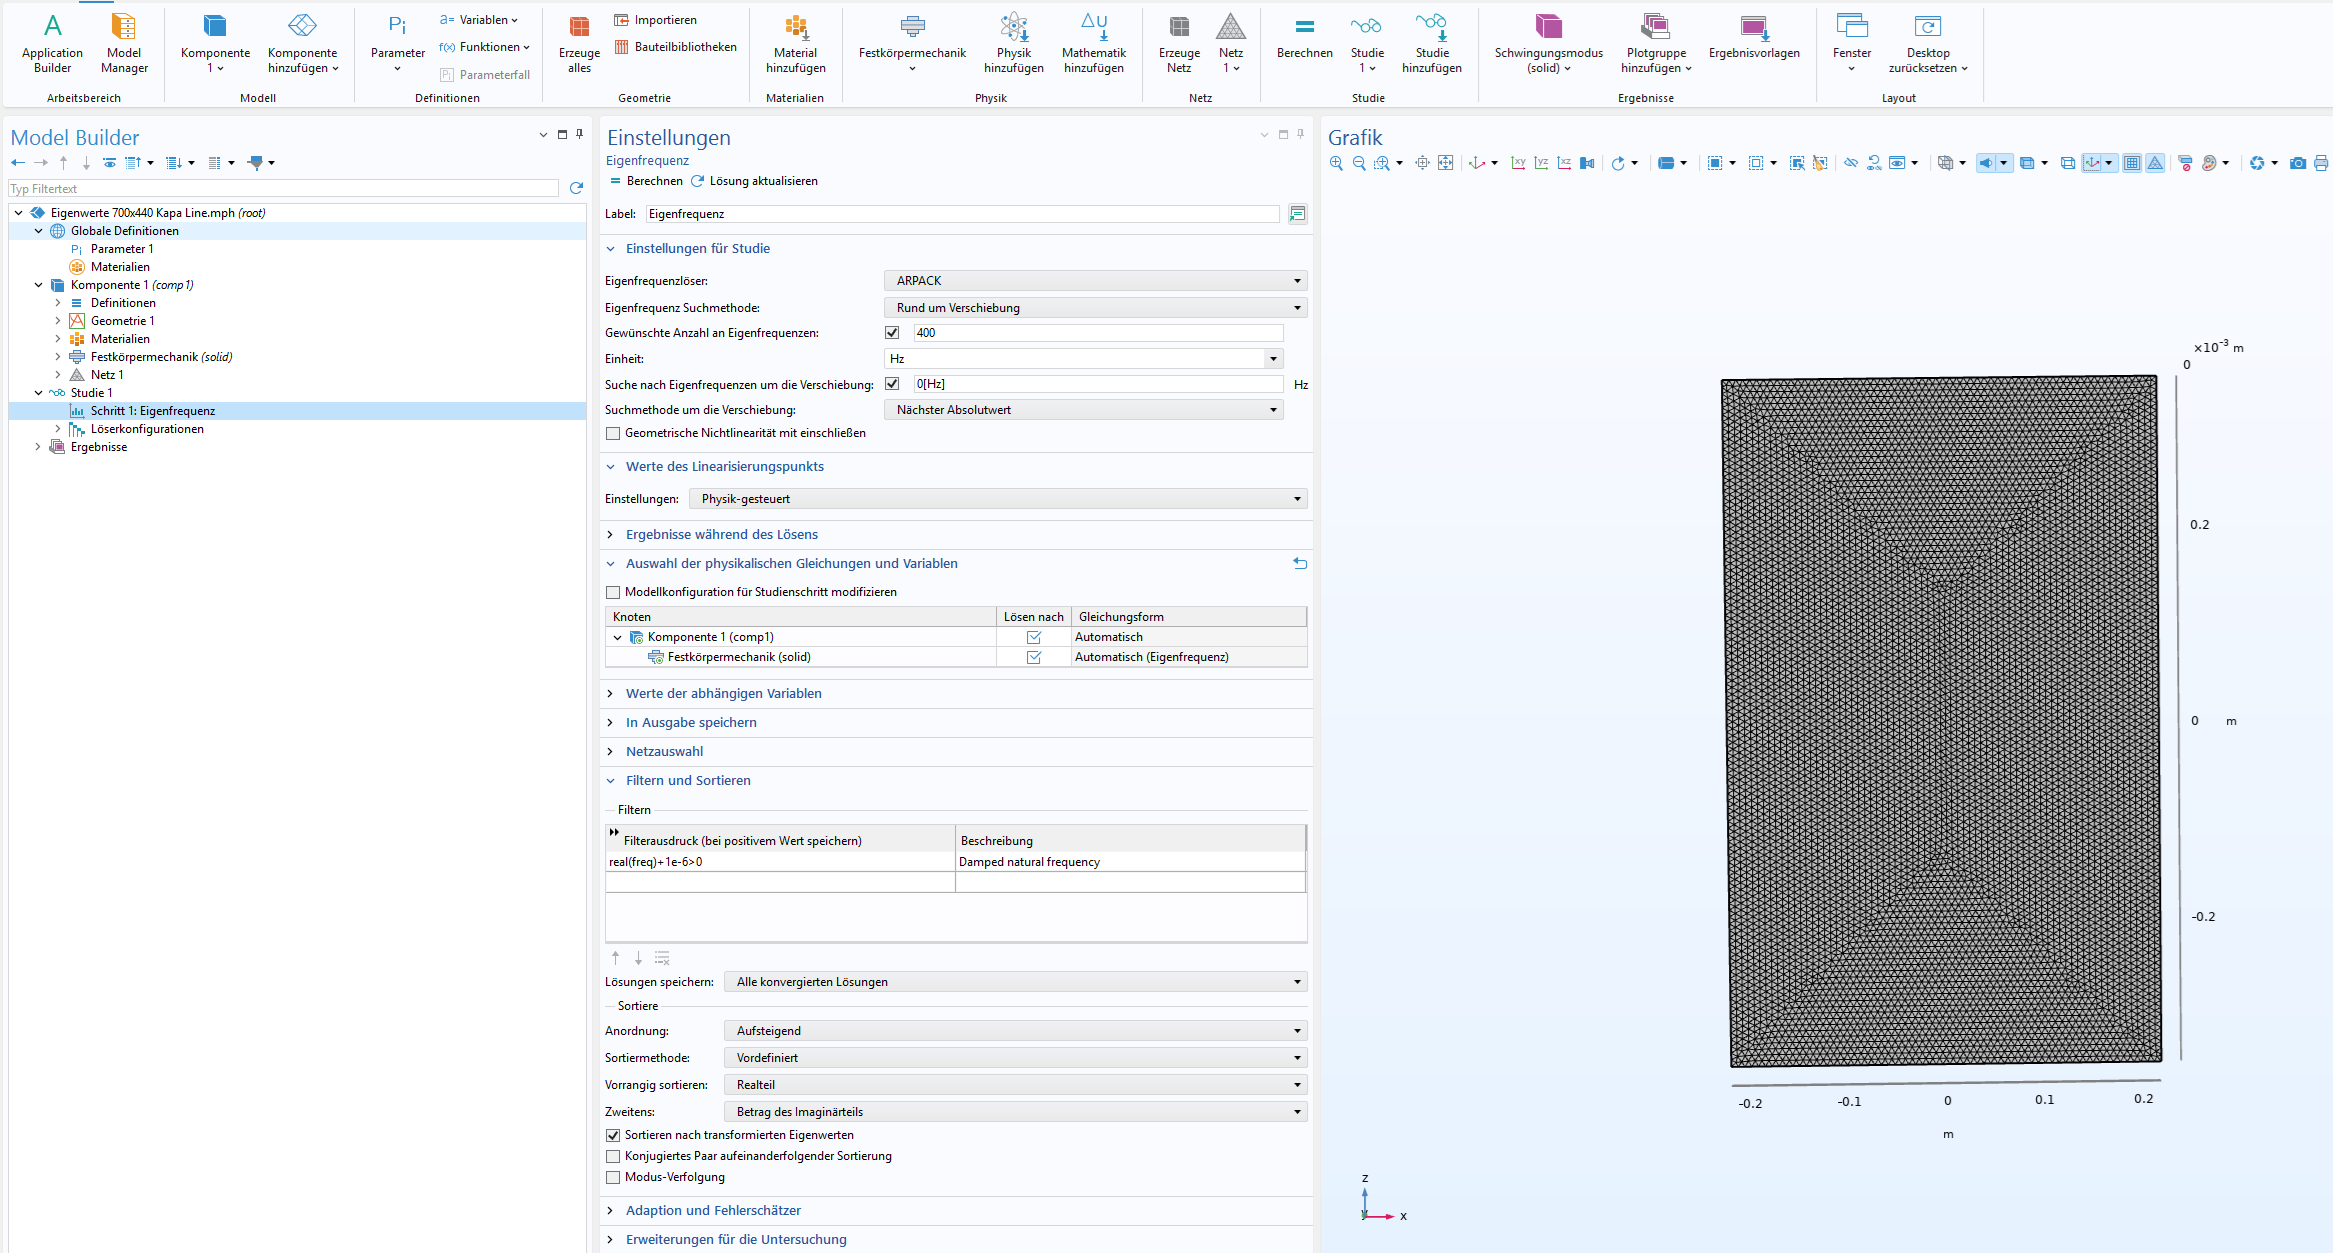
\includegraphics[width=0.8\textwidth]{pictures/Modellaufbau.png}
	\caption{Modellaufbau der DML-Platte in COMSOL Multiphysics}
	\label{fig:modellaufbau}
\end{figure}


Die Abbildung \ref{fig:modellaufbau} zeigt den Modellaufbau der Platte, zu sehen ist die Platte, welche mit einem Netz bespannt ist. In der Studie ist die gewünschte Anzahl der Eigenfrequenzen auf 400 eingestellt und die Berechnung startet bei 0 Hz und endet, wenn 400 Eigenmoden der Platte berechnet wurden. 




\subsection{Durchgeführte Simulationsstudien und Ergebnisse}

Die berechneten Eigenmoden der Platten bilden Muster, welche die Verschiebung der Platte bei den Eigenfrequenzen zeigen. Die Abbildungen zeigen die Muster der simulierten Eigenmoden um die Frequenzen bei \SI{50}{\hertz}, \SI{150}{\hertz}, \SI{300}{\hertz}, \SI{500}{\hertz}, \SI{800}{\hertz} und \SI{1000}{\hertz} an.  

\begin{figure}[H]
	\centering
	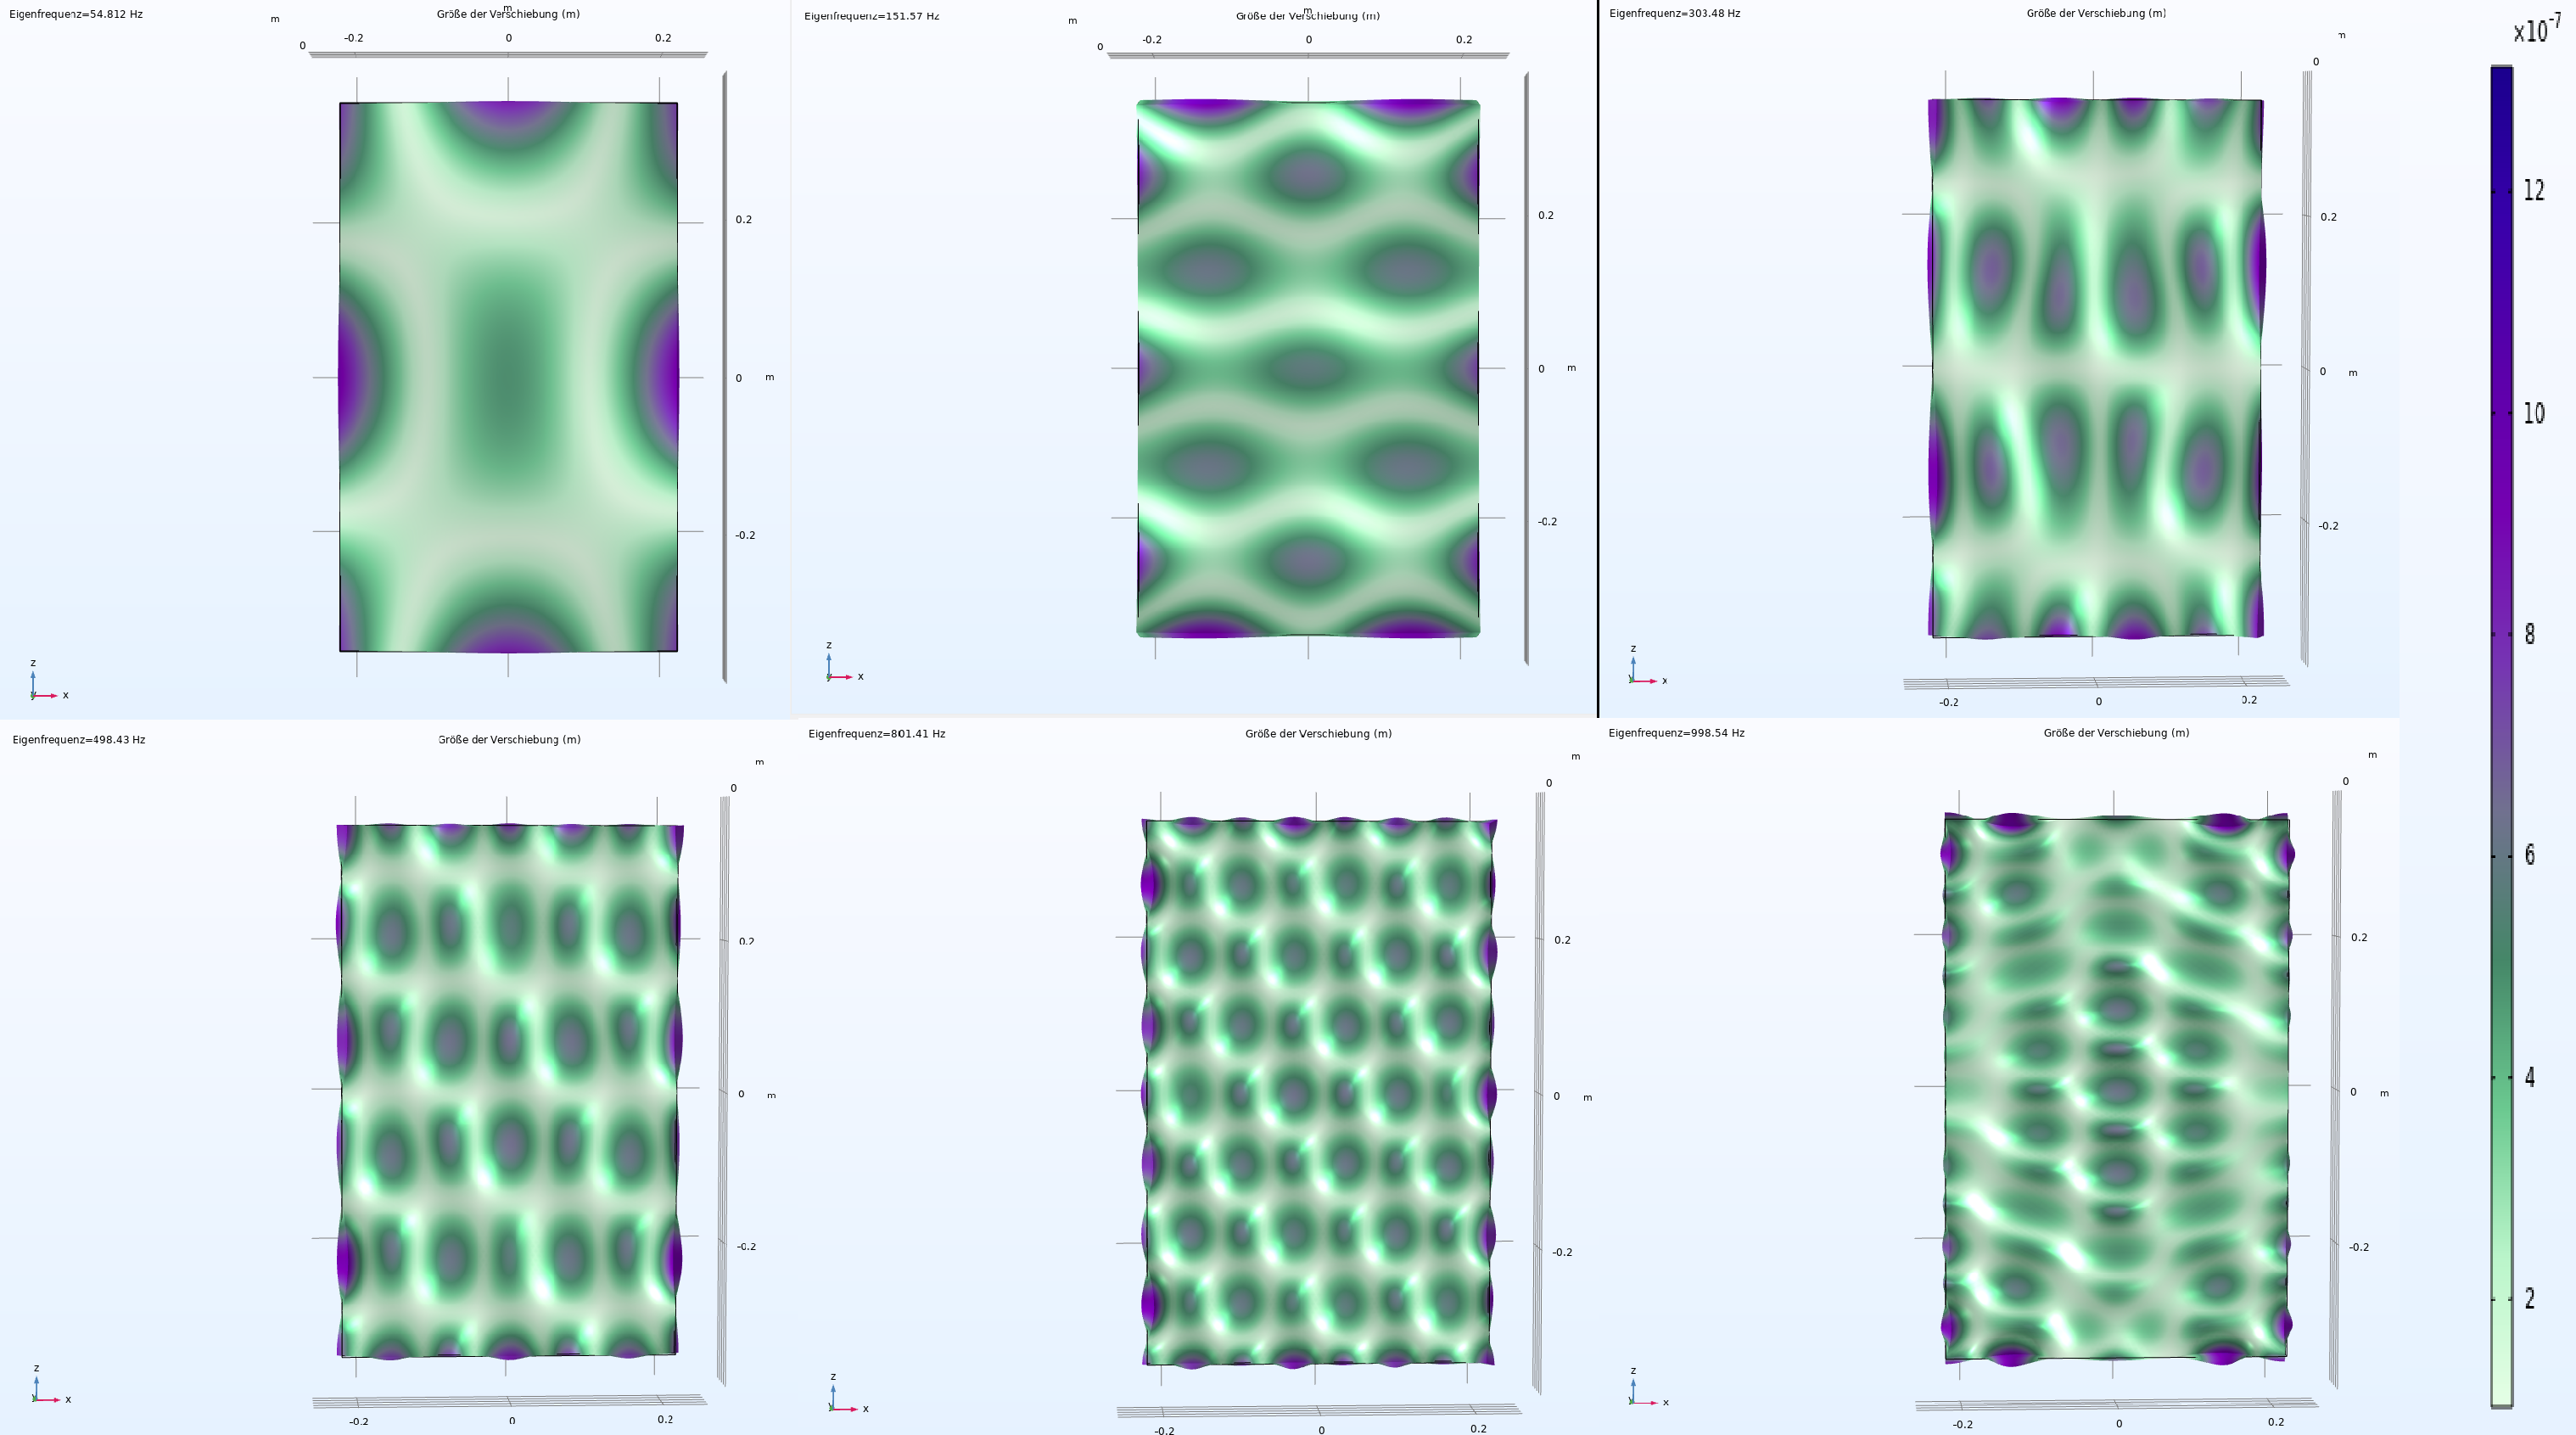
\includegraphics[width=0.9\textwidth]{pictures/Eigenmoden_0.7m.png}
	\caption{Eigenmoden der KAPA Line Platte (\SI{0,7}{\meter} x \SI{0,44}{\meter})}
	\label{fig:eigenmoden_07m}
\end{figure}

\begin{figure}[H]
	\centering
	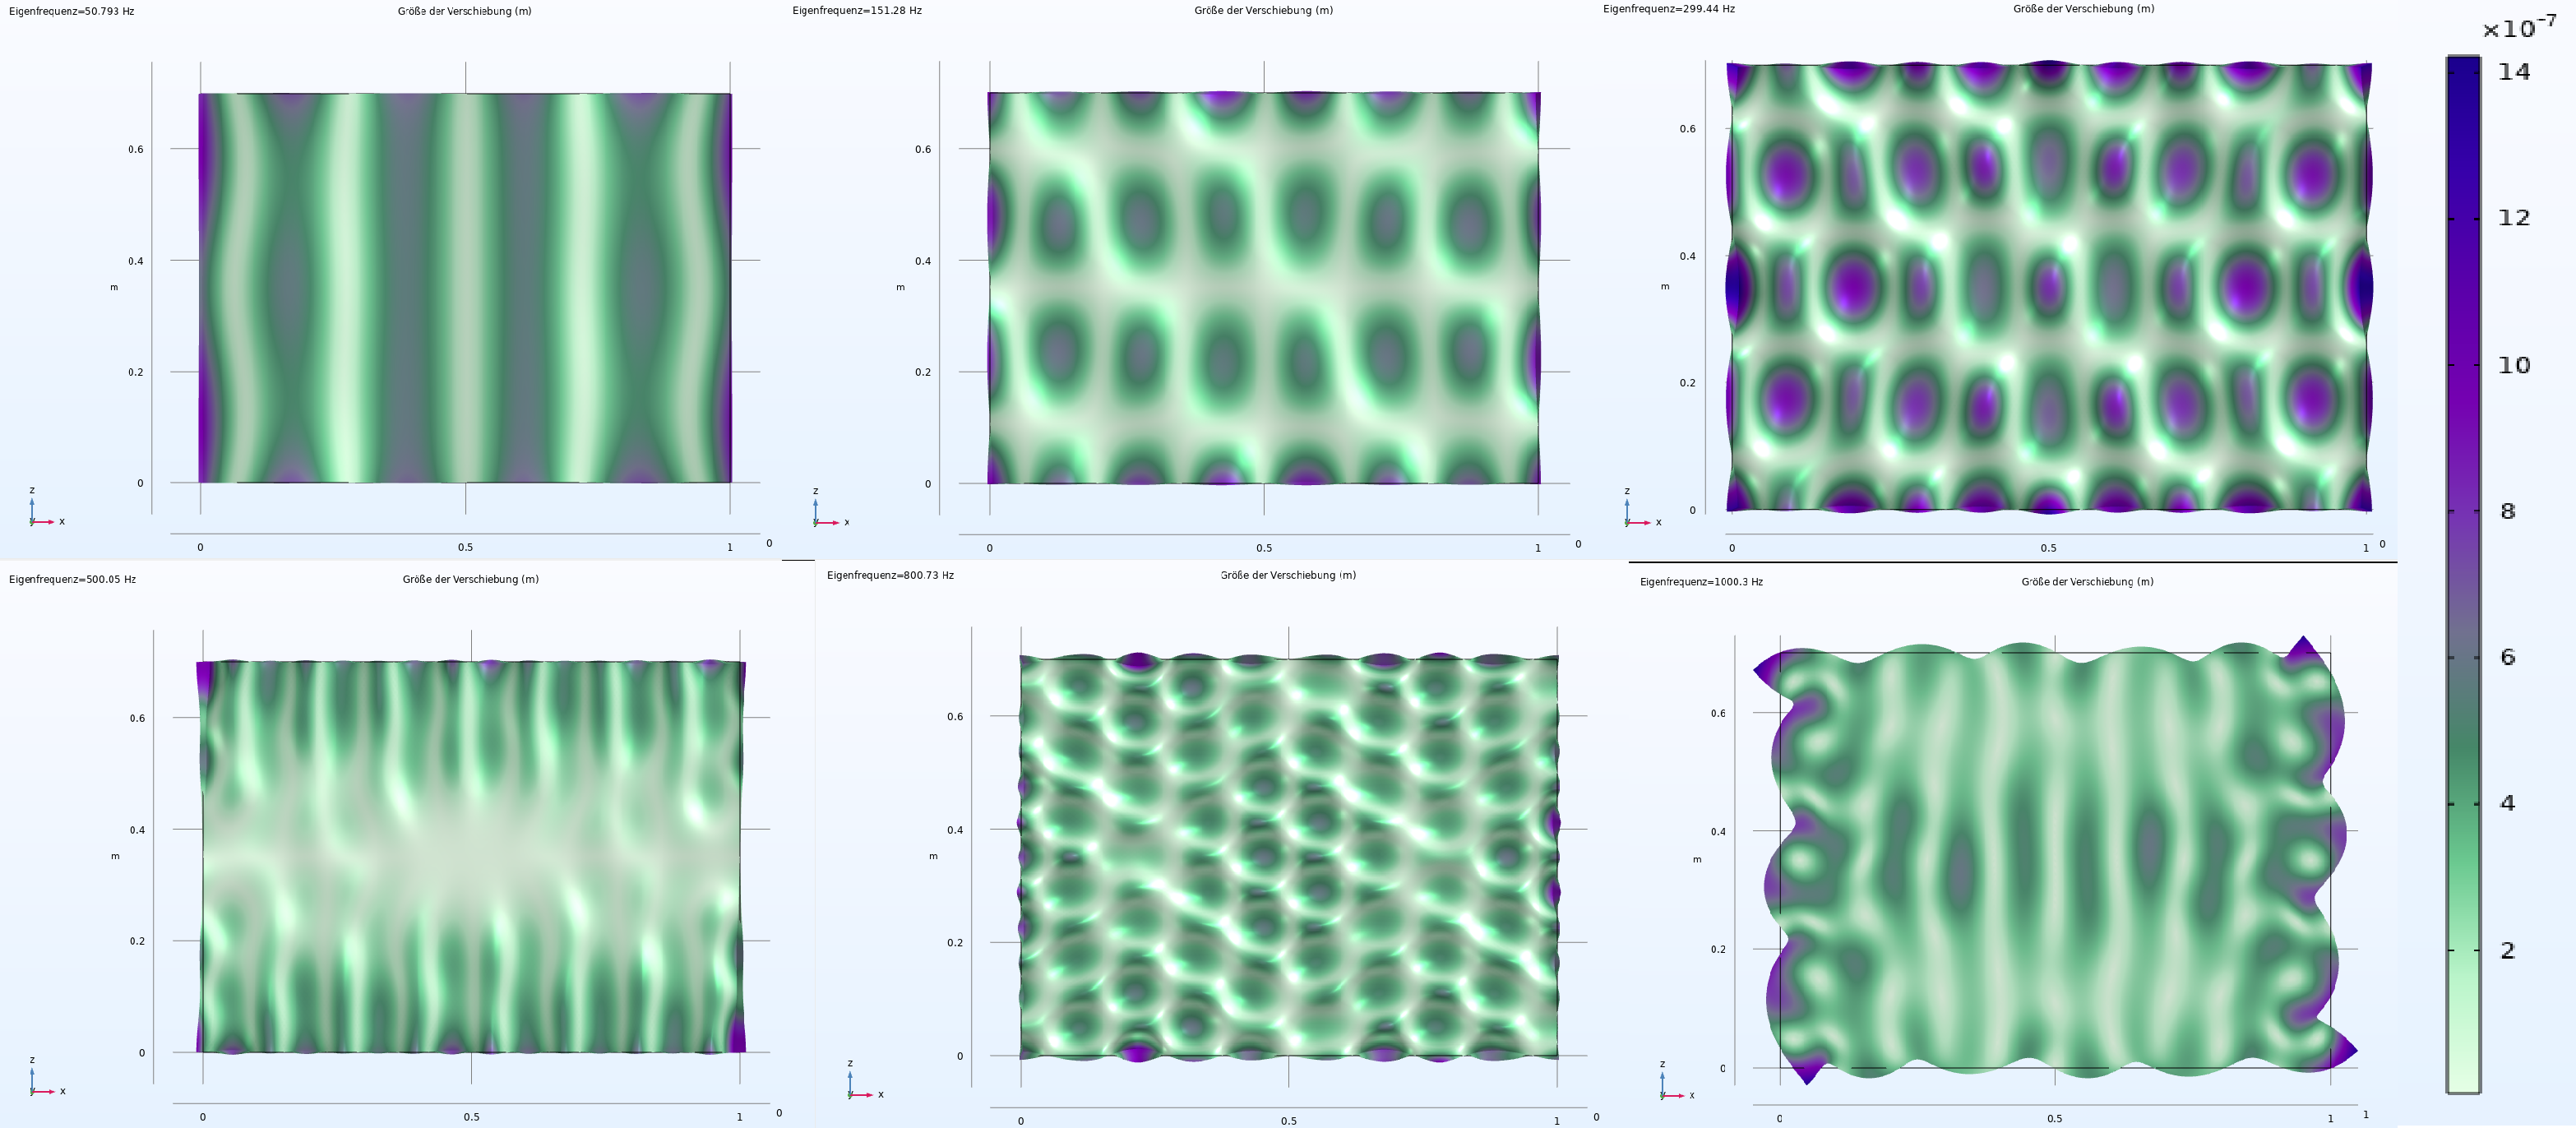
\includegraphics[width=0.9\textwidth]{pictures/Eigenmoden_1m.png}
	\caption{Eigenmoden der KAPA Line Platte (\SI{1}{\meter} x \SI{0,7}{\meter})}
	\label{fig:eigenmoden_1m}
\end{figure}

Die Legende, welche in den Abbildungen \ref{fig:eigenmoden_07m} und \ref{fig:eigenmoden_1m} auf der rechten Seite zu sehen ist, zeigt an, dass die dunklen violetten Bereiche eine größere Verschiebung aufweisen. Je heller die Platte, desto weniger Verschiebung. 

Die Plattenverschiebung bei den Eigenfrequenzen wird in der Auswertung genutzt, um die Positionen der Exciter zu bestimmen. Hierfür wurden die Daten der Simulation in Abhängigkeit zu einer durch die Mitte der Platte verlaufenden Referenzebene exportiert. Dabei wurde ein Raster über die Platte zur Auswertung der einzelnen Punkte gelegt. Anschließend wurden die Daten in einem Python-Skript anhand ihrer Verschiebung ausgewertet. Dabei wurden Punkte, an denen eine geringe Verschiebung auftritt, als gut und dort, wo eine hohe Verschiebung auftritt, als schlecht bewertet. Anhand dieser Bewertung wurde die ideale Position für zwei Exciter auf der Platte bestimmt. 


\clearpage

\section{Realer Versuchsaufbau}

In diesem Kapitel wird der Versuchsaufbau zur Vermessung der akustischen Eigenschaften der DML-Lautsprecher beschrieben, realisiert und durchgeführt. Zur Durchführung der Messungen sowie zur Signalverarbeitung wird die Software LabVIEW der Firma National Instruments eingesetzt. Der Aufbau des in LabVIEW geschriebenen Programms mit dem das Testsignal generiert wird, dient auch der Erfassung und Weiterverarbeitung der Messdaten und wird in den Folgekapiteln beschrieben.
Der Versuchsaufbau verfolgt hierbei zwei primäre Ziele, die Erfassung des Frequenzgangs des DML-Lautsprechers der verschiedenen Exciterpositionen sowie die Darstellung des Schallfeldes des DML. 

 
\subsection{LabVIEW}
LabVIEW ist ein Programm der Firma National Instruments, mit dem sich in einer grafischen Entwicklungsumgebung Mess-, Steuer-, Regel- und Automatisierungssysteme programmieren lassen. Statt textbasiertem Code verwendet LabVIEW Blockdiagramme zur Datenverarbeitung
Für die Vermessung der akustischen Eigenschaften des DML-Lautsprechers und dessen Beurteilung muss das in LabVIEW geschriebene Programm die folgenden Funktionen umfassen: 

\begin{itemize}
    \item Erzeugen und Abspielen eines Testsignals 
    \item Erfassung des Mikrofon- und Referenzsignals
    \item Verarbeitung der Messwerte und Bilden der Übertragungsfunktion
    \item Darstellung der Messwerte in einem Graphen
    \item Speichern der Messwerte als verarbeitbare Datei.
\end{itemize}

 Ein LabVIEW-Programm besteht dabei aus zwei wesentlichen Bestandteilen. Der Benutzeroberfläche, dem Frontpanel, und einer Funktionslogik, auch Blockdiagramm genannt. Im Blockdiagramm werden virtuelle Instrumente, kurz VI, verwendet, um Signale zu erzeugen oder zu bearbeiten, Daten zu erfassen, Systeme zu regeln oder zu steuern. Die einzelnen VIs lassen sich im grafischen Programmcode mit verschiedenen Drähten verbinden. Diese sind farbcodiert und können jeweils nur eine bestimmte Art von Daten übermitteln. Mittels der Drähte lässt sich der Datenfluss und damit der Ablauf der einzelnen Programmschritte festlegen.  

In dieser Arbeit wird LabVIEW verwendet, um den DML-Lautsprecher auf seine akustischen Eigenschaften zu untersuchen. Dabei wird ein Audiosignal in LabVIEW erzeugt und über den DAQ-OUTPUT an den Audioverstärker geleitet und über den DML-Lautsprecher abgespielt. Das Signal wird akustisch wiedergegeben und von einem Messmikrofon empfangen. Die dabei entstehende Übertragungsfunktion gibt Erkenntnisse über die Effizienz und den Schalldruckpegel des Lautsprechers. Das Signal vom Messmikrofon wird wieder in den DAQ-INPUT geleitet und in LabVIEW ausgewertet. 


\begin{figure}[H]
	\centering
	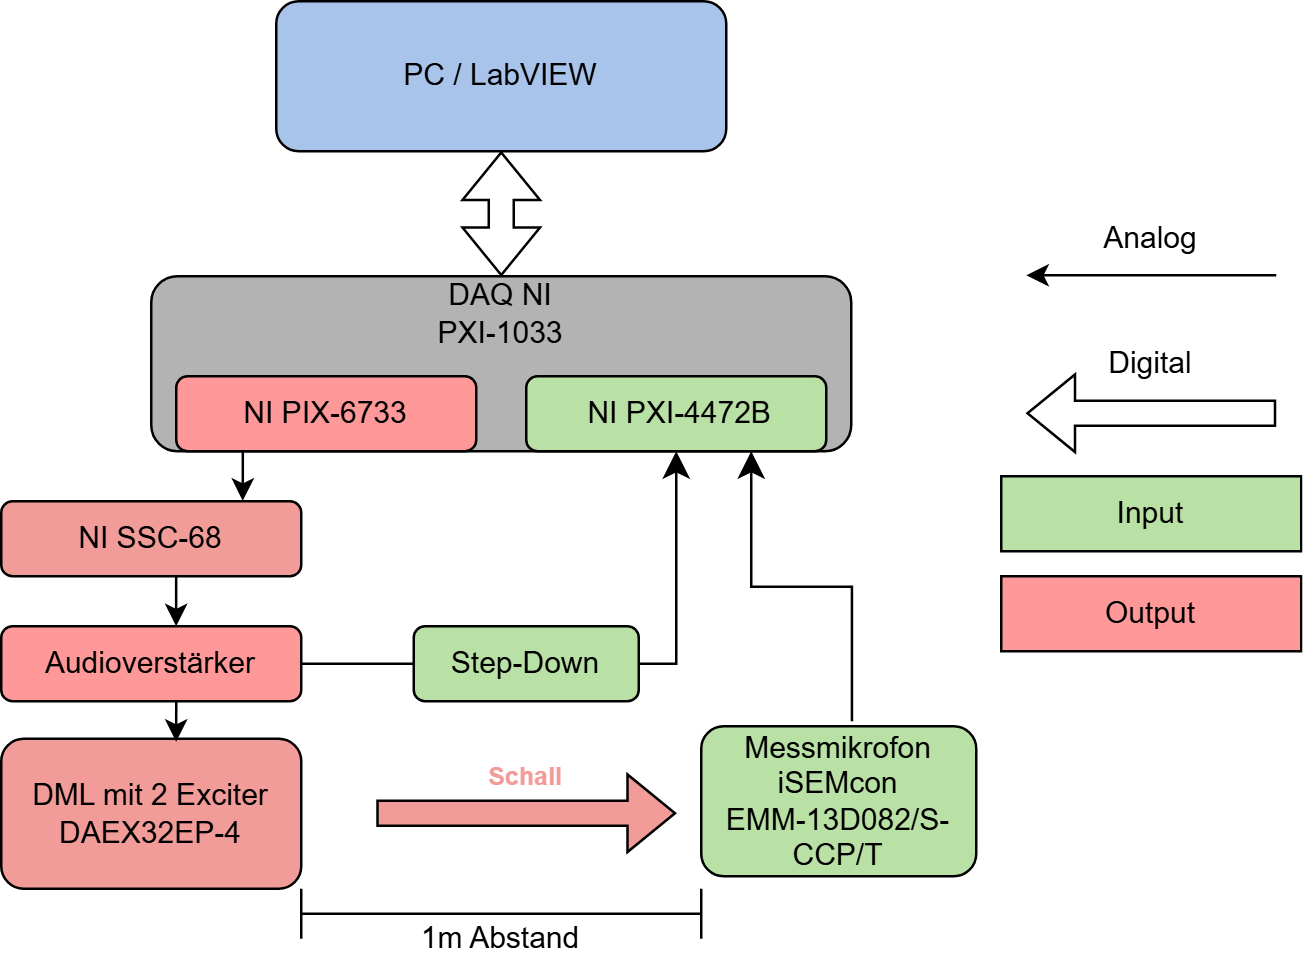
\includegraphics[width=0.6\textwidth]{pictures/Blockschaltbild LabVIEW.png}
	\caption{Versuchsaufbau DML-Lautsprecher Vermessen}
	\label{fig:blockschaltbild_exciter}
\end{figure}

Abbildung \ref{fig:blockschaltbild_exciter} zeigt den Signalfluss des Versuchsaufbaus im Freifeldraum in Form eines Blockschaltbildes. Als Testsignal wird in LabVIEW ein weißes Rauschen erzeugt, das über den Ausgang der NI PXI-6733 Datenausgabekarte an den Audioverstärker weitergeleitet wird. Das vom Verstärker verstärkte elektrische Signal wird anschließend über den Lautsprecherausgang sowohl an die verwendeten Exciter als auch an einen Step-Down-Converter geführt.
Der Step-Down-Converter reduziert die Spannung des Verstärkerausgangssignals und stellt ein Referenzsignal bereit, das zur Bestimmung der Übertragungsfunktion verwendet wird. Dieses Referenzsignal wird auf einen Eingang der NI PXI-4472B Datenerfassungskarte geführt. Parallel dazu wandeln die Exciter das verstärkte elektrische Signal in mechanische Schwingungen um, wodurch das DML-Panel angeregt wird und Schallwellen erzeugt.
Die abgestrahlten Schallwellen werden vom Messmikrofon aufgenommen und in ein elektrisches Signal umgewandelt. Dieses Mikrofonsignal wird ebenfalls auf einen Eingang der NI PXI-4472B Datenerfassungskarte geleitet. Somit liegen sowohl das Referenzsignal als auch das Messsignal gleichzeitig in digitaler Form vor.
Die erfassten Eingangssignale werden in LabVIEW umgerechnet und gemittelt, sodass aus dem Referenz- und Messsignal die frequenzabhängige Übertragungsfunktion des Lautsprechers bestimmt werden kann. Dadurch ist eine objektive Bewertung des Frequenzgangs sowie des Schalldruckpegels unter definierten Freifeldbedingungen möglich.


\subsection{Blockdiagramm und Signalverarbeitung}

Das Blockschaltbild in LabVIEW stellt die Datenerzeugung und -verarbeitung dar und kann als Ablaufplan angesehen werden. Das Blockschaltbild besteht dabei aus verschiedenen VIs, welche nacheinander ausgeführt und deren Zustände ermittelt werden. In diesem Programm ist die „While-Schleife" der Kern des Programms, da diese Abfolge Periodisch ist, bis eine Bedingung erfüllt ist. Mit dieser Schleife können die aufgenommenen Werte gemittelt werden. Das Programm für die Vermessung des DML-Lautsprechers hat folgenden Aufbau:

\begin{enumerate}
    \item Initialisierung der Ein- und Ausgangskanäle
    \item Erzeugen eines Testsignals 
    \item Empfangen der Eingangssignale
    \item Verarbeitung der Signale
    \item Mittelung der Signale
    \item Darstellung der Signale
\end{enumerate}


 Vor der While-Schleife werden Parameter mittels Bedienelement erstellt. Dazu zählen die Input- und Output-Kanäle des DAQ und die Mikrofonempfindlichkeit des verwendeten Mikrofons, welche aus dem Datenblatt im Anhang YX entnommen werden kann. Zusätzlich lassen sich die Abtastparameter bestimmen, diese bestimmen die Blockgröße und Anzahl der Mittelungen. Die Anzahl der pro Datenblock verarbeiteten Abtastwerte ergibt sich aus der Abtastfrequenz fs und der Blocklänge N.
 
 \begin{equation}
\Delta f = \frac{f_s}{N}
\end{equation}

Wobei $\Delta f$ die Frequenzauflösung des Spektrums in Hz, $f_s$ die Abtastfrequenz in Hz und $N$ die Anzahl der Abtastwerte pro Datenblock ist. 



Abbildung Whileschleife.PNG


In der Whileschleife wird das weiße Rauschen erzeugt, die Eingangssignale erfasst und verarbeitet sowie grafisch dargestellt. 

Das Weiße Rauschen wird über die Outputkarte NI PXI-6733 welche im Steckplatz 2 des DAQ NI PXI-1033 steckt, ausgegeben. Dafür wird die OutputBox NI SCC-68 verwendet welche einen Cinch-Anschluss am Output 22 und 54 angeschlossen hat. Das weiße Rauschen wird mit Hilfe des Uniform White Noise Waveform VI generiert.

Das Eingangssignal von der NI PXI-4472B welche im Steckplatz 1 des DAQ NI PXI-1033 steckt, ist anfangs gebündelt und wird mittels Index Array VI in das Referenzsignal und das Mikrofonsignal separiert.
Aus den beiden Signalen lässt sich mittels Frequency Response VI die Übertragungsfunktion, sowie die zugehörige Kohärenz berechnen. 
Die zugehörigen komplexen Spektren werden als $X[k]$, Referenzsignal und $Y[k]$, Mikrofonsignal bezeichnet.
Für die Übertragungsfunktion wird der $H_1$-Schätzer verwendet. Dieser basiert auf dem Kreuzspektrum zwischen Eingangs- und Ausgangssignal sowie dem Autospektrum des Eingangssignals und minimiert den Einfluss von Störungen am Ausgangssignal:

\begin{equation}
H_1[k] = \frac{G_{xy}[k]}{G_{xx}[k]}
\end{equation}

wobei $H_1[k]$ der $H_1$-Schätzer der Übertragungsfunktion, $G_{xy}[k]$ das Kreuzspektrum zwischen Referenz- und Antwortsignal und $G_{xx}[k]$ das Autospektrum des Referenzsignals ist.
Der FRF-Graph beschreibt die relative frequenzabhängige Systemantwort des gesamten Aufbaus aus Verstärker, Exciter, DML-Platte und Schallabstrahlung. Der FRF-Graph dient insbesondere der Beurteilung von Resonanzen, Einbrüchen und der relativen Linearität des Systems, dabei ist dieser immer unter Berücksichtigung der Kohärenz zu betrachten. Die Kohärenz gibt an wie gut das Eingangssignal das Ausgangssignal widerspiegelt. Die Kohärenz wird in einem Wertebereich von 0 bis 1 angezeigt. Werte nahe 1 zeigen, dass das Ausgangssignal der jeweiligen Frequenz vollständig durch das Eingangssignal erklärt wird.


Parallel zur Berechnung der Übertragungsfunktion wird der Schalldruckpegel des Lautsprechers berechnet. Der SPL-Graph zeigt den absoluten Schalldruckpegel am Mikrofon über der Frequenz und dient vor allem zur Bewertung der tatsächlich erreichten Lautstärke und wie sich die Übertragungsfunktion verhält.
Dafür wird das Signal mittels Fast Fourier Transformation (kurz FFT) VI in den Frequenzbereich transformiert. Nach der Transformation wird aus dem komplexen Schalldruckspektrum das lineare Amplitudenspektrum berechnet.   





%Das in LabVIEW erzeugte diskrete Anregungssignal kann allgemein als Folge $x[n]$ beschrieben werden. Die Anzahl der pro Datenblock verarbeiteten Abtastwerte ergibt sich aus der Abtastfrequenz $f_s$ und der Blocklänge $N$. Die zugehörige Frequenzauflösung der späteren Spektralanalyse ergibt sich zu

%\begin{equation}
%\Delta f = \frac{f_s}{N}
%\end{equation}

%wobei $\Delta f$ die Frequenzauflösung des Spektrums in Hz, $f_s$ die Abtastfrequenz in Hz und $N$ die Anzahl der Abtastwerte pro Datenblock ist.

%Das Referenzsignal wird elektrisch am Verstärkerausgang abgegriffen, mittels Step-Down-Wandler auf einen zulässigen Messbereich reduziert und anschließend als Spannungssignal $x_{\mathrm{ref}}[n]$ in den DAQ eingelesen. Das Mikrofon liefert ebenfalls ein Spannungssignal $u_{\mathrm{mic}}[n]$, welches proportional zum auftretenden Schalldruck ist. Für das verwendete Messmikrofon beträgt die Empfindlichkeit laut Kalibrierblatt $S = 0{,}028\;\mathrm{V/Pa}$. Wird keine zusätzliche externe lineare Vorverstärkung berücksichtigt, so kann für den Verstärkungsfaktor $G = 1$ gesetzt werden. Die Umrechnung des gemessenen Mikrofonsignals von Volt in Pascal erfolgt damit gemäß

%\begin{equation}
%p[n] = \frac{u_{\mathrm{mic}}[n]}{S \cdot G}
%\end{equation}

%wobei $p[n]$ das Schalldrucksignal im Zeitbereich in Pa, $u_{\mathrm{mic}}[n]$ die gemessene Mikrofonspannung im Zeitbereich in V, $S$ die Mikrofonempfindlichkeit in V/Pa und $G$ der lineare Verstärkungsfaktor der Messkette ist.

%Für das verwendete Mikrofon und ohne zusätzliche externe Verstärkung vereinfacht sich die Gleichung zu

%\begin{equation}
%p[n] = \frac{u_{\mathrm{mic}}[n]}{0{,}028}
%\end{equation}

%Um bei der blockweisen Verarbeitung Spektralleckeffekte (Spectral Leakage) zu minimieren, wird vor der Fourier-Transformation auf jeden Datenblock eine Fensterfunktion angewendet. Im vorliegenden Messaufbau wird ein Hanning-Fenster verwendet. Das gefensterte Signal ergibt sich zu

%\begin{equation}
%p_w[n] = p[n] \cdot w[n]
%\end{equation}

%wobei $p_w[n]$ das gefensterte Schalldrucksignal, $p[n]$ das Schalldrucksignal im Zeitbereich und $w[n]$ die Fensterfunktion (hier: Hanning-Fenster) ist.

%Nach der Fensterung wird das Signal blockweise in den Frequenzbereich transformiert. Hierzu wird die diskrete Fourier-Transformation (DFT) verwendet:

%\begin{equation}
%P[k] = \sum_{n=0}^{N-1} p_w[n] \cdot e^{-j \cdot \frac{2\pi k n}{N}}
%\end{equation}

%wobei $P[k]$ das komplexe Schalldruckspektrum, $p_w[n]$ das gefensterte Schalldrucksignal im Zeitbereich, $N$ die Anzahl der Abtastwerte, $n$ der Zeitindex, $k$ der Frequenzindex und $j$ die imaginäre Einheit ist.

%Aus dem komplexen Spektrum wird anschließend das einseitige lineare Amplitudenspektrum berechnet. Da bei reellwertigen Signalen das Spektrum symmetrisch ist, wird nur der Bereich $0 \leq k \leq N/2$ ausgewertet. Die Normierung auf die Blocklänge und die Berücksichtigung der Energieverteilung auf beide Spektrumshälften ergibt:

%\begin{equation}
%A[k] = \frac{2 \cdot |P[k]|}{N} \quad \text{für } 1 \leq k \leq \frac{N}{2} - 1
%\end{equation}

%\begin{equation}
%A[0] = \frac{|P[0]|}{N} \quad \text{(Gleichanteil)}
%\end{equation}

%\begin{equation}
%A\left[\frac{N}{2}\right] = \frac{\left|P\left[\frac{N}{2}\right]\right|}{N} \quad \text{(Nyquist-Frequenz)}
%\end{equation}

%wobei $A[k]$ das einseitige lineare Amplitudenspektrum in Pa, $|P[k]|$ der Betrag des komplexen Spektrums und $N$ die Anzahl der Abtastwerte ist.

%Der Faktor 2 kompensiert, dass bei der einseitigen Darstellung die Energie der negativen Frequenzanteile den positiven zugeschlagen wird. Die Sonderfälle $k = 0$ (Gleichanteil) und $k = N/2$ (Nyquist-Frequenz) werden ohne den Faktor 2 normiert, da diese Frequenzanteile im zweiseitigen Spektrum nicht gespiegelt auftreten.

%Da bei der Messung eine Mittelung über mehrere Datenblöcke durchgeführt wird, werden zunächst die linearen Amplitudenspektren aufsummiert und anschließend gemittelt. Für $M$ Mittelungen ergibt sich:

\begin{equation}
\bar{A}[k] = \frac{1}{M} \cdot \sum_{i=1}^{M} A_i[k]
\end{equation}

wobei $\bar{A}[k]$ das gemittelte lineare Amplitudenspektrum, $M$ die Anzahl der Mittelungen und $A_i[k]$ das lineare Amplitudenspektrum des $i$-ten Datenblocks ist.

Die Darstellung des Schalldruckpegels über der Frequenz erfolgt anschließend in dB SPL. Dazu wird das gemittelte lineare Spektrum auf den Bezugsdruck $p_0 = 20\;\mu\mathrm{Pa}$ normiert:

\begin{equation}
L_p[k] = 20 \cdot \log_{10}\left(\frac{\bar{A}[k]}{p_0}\right)
\end{equation}

wobei $L_p[k]$ der Schalldruckpegel in dB SPL, $\bar{A}[k]$ das gemittelte lineare Amplitudenspektrum in Pa und $p_0 = 20 \cdot 10^{-6}\;\mathrm{Pa}$ der Bezugsdruck ist.

Setzt man den Bezugsdruck explizit ein, ergibt sich:

\begin{equation}
L_p[k] = 20 \cdot \log_{10}\left(\frac{\bar{A}[k]}{20 \cdot 10^{-6}}\right)
\end{equation}

Parallel zur SPL-Berechnung wird aus Referenzsignal und akustischer Antwort die Übertragungsfunktion des Systems bestimmt. Dazu werden das Referenzsignal $x_{\mathrm{ref}}[n]$ sowie das Schalldrucksignal $p[n]$ ebenfalls gefenstert und in den Frequenzbereich transformiert. Die zugehörigen komplexen Spektren werden als $X[k]$ (Referenz) und $Y[k]$ (Antwort) bezeichnet.

Zur robusten Schätzung der Übertragungsfunktion wird der $H_1$-Schätzer verwendet. Dieser basiert auf dem Kreuzspektrum zwischen Eingangs- und Ausgangssignal sowie dem Autospektrum des Eingangssignals und minimiert den Einfluss von Störungen am Ausgangssignal:

\begin{equation}
H_1[k] = \frac{G_{xy}[k]}{G_{xx}[k]}
\end{equation}

wobei $H_1[k]$ der $H_1$-Schätzer der Übertragungsfunktion, $G_{xy}[k]$ das Kreuzspektrum zwischen Referenz- und Antwortsignal und $G_{xx}[k]$ das Autospektrum des Referenzsignals ist.

Dabei berechnen sich die gemittelten Spektren über $M$ Blöcke zu:

\begin{equation}
G_{xy}[k] = \frac{1}{M} \cdot \sum_{i=1}^{M} X_i^*[k] \cdot Y_i[k]
\end{equation}

\begin{equation}
G_{xx}[k] = \frac{1}{M} \cdot \sum_{i=1}^{M} |X_i[k]|^2
\end{equation}

wobei $X_i^*[k]$ das konjugiert komplexe Spektrum des Referenzsignals im $i$-ten Block, $Y_i[k]$ das komplexe Spektrum des Antwortsignals im $i$-ten Block und $M$ die Anzahl der gemittelten Blöcke ist.

Zur Darstellung des Betrags der Übertragungsfunktion in Dezibel wird verwendet:

\begin{equation}
H_{\mathrm{dB}}[k] = 20 \cdot \log_{10}\left(|H_1[k]|\right)
\end{equation}

wobei $H_{\mathrm{dB}}[k]$ der Betrag der Übertragungsfunktion in dB und $|H_1[k]|$ der Betrag des $H_1$-Schätzers ist.

Der FRF-Graph beschreibt somit die relative frequenzabhängige Systemantwort des gesamten Aufbaus aus Verstärker, Exciter, DML-Platte und Schallabstrahlung. Im Gegensatz dazu zeigt der SPL-Graph den absoluten Schalldruckpegel am Mikrofon über der Frequenz. Während der SPL-Graph vor allem zur Bewertung der tatsächlich erreichten Lautstärke und des nutzbaren Übertragungsbereichs geeignet ist, dient der FRF-Graph insbesondere der Beurteilung von Resonanzen, Einbrüchen und der relativen Linearität des Systems.

Zur qualitativen Beurteilung der Messgüte wird zusätzlich die Kohärenz zwischen Referenz- und Antwortsignal berechnet. Die Kohärenzfunktion gibt an, in welchem Maß das Ausgangssignal linear mit dem Eingangssignal zusammenhängt. Sie ergibt sich aus den gemittelten Auto- und Kreuzspektren zu:

\begin{equation}
\gamma^2[k] = \frac{|G_{xy}[k]|^2}{G_{xx}[k] \cdot G_{yy}[k]}
\end{equation}

wobei $\gamma^2[k]$ die Kohärenzfunktion (Wertebereich 0 bis 1), $G_{xy}[k]$ das Kreuzspektrum zwischen Eingangs- und Ausgangssignal, $G_{xx}[k]$ das Autospektrum des Referenzsignals und $G_{yy}[k]$ das Autospektrum des Antwortsignals ist.

Ein Kohärenzwert nahe 1 zeigt an, dass das Ausgangssignal bei der jeweiligen Frequenz vollständig durch das Eingangssignal erklärt wird. Werte deutlich unter 1 deuten auf nichtlineare Effekte, Störgeräusche oder eine unzureichende Anregung bei der betreffenden Frequenz hin.

\clearpage

 \subsection{Durchführung der Messungen}
 
 Um die durchgeführten Messungen vergleichen zu können, wurden während des gesamten Versuchsaufbaus die Einstellungen des Equalizers und des Audioverstärkers nicht geändert. Die genauen Einstellungen können dem Anhang XY entnommen werden, der Equalizer hat während der Messungen keine Signalanpassung vorgenommen.

Der erste Versuchsaufbau dient der Erfassung von den akustischen Eigenschaften des DML, hierbei werden verschiedene Plattengrößen und jeweils unterschiedliche Exciter-Positionen vermessen. Verglichen werden die Ergebnisse aus der Simulation, Kapitel 3.3.3 und die vom Hersteller angegebenen Positionen für die Exciter, Anhang A.
Zur Vermessung werden die Platten im Freifeldraum an Schnüren aufgehängt. Das Messmikrofon wird einen Meter vor der Plattenmitte positioniert.

\begin{figure}[H]
	\centering
	\includegraphics[width=0.7\textwidth]{pictures/Versuchsaufbau.png}
	\caption{Messaufbau im Freifeldraum}
	\label{fig:messaufbau_freifeldraum}
\end{figure}

Die Abbildung \ref{fig:messaufbau_freifeldraum} zeigt den Versuchsaufbau im Freifeldraum, der DML-Lautsprecher wurde dabei freihängend aufgehängt und das Messmikrofon mit einem Arm von der Decke auf einem Meter Abstand fest montiert.


Das Ziel des zweiten Versuchsaufbaus ist die Erfassung des abgestrahlten Schallfeldes des Lautsprechers. Für diesen Aufbau wurde die Position des Messmikrofons nicht verändert. Die Platte wurde mittig an einer in den PUR-Hartschaum geklebten Öse drehbar aufgehängt. An den beiden unteren Ecken der Platte sind Schnüre angebracht, welche am Boden an einer Wasserwaage befestigt sind. Am Boden sind mit Klebeband Markierungen der Messpunkte alle 15 Grad aufgeklebt.

\begin{figure}[H]
	\centering
	\includegraphics[width=0.7\textwidth]{pictures/Schallfeld_messung.png}
	\caption{Versuchsaufbau zur Schallfeldmessung}
	\label{fig:schallfeld_messung}
\end{figure}

Die Abbildung \ref{fig:schallfeld_messung} zeigt den beschriebenen Aufbau. Die Wasserwaage dient als Gewicht um die Platte gerade zu ziehen. Zur Ausrichtung der Platte wurde ein Laser verwendet, der grüne Laser ist mittig auf der Platte und an der Unterseite des Messmikrofons in Abbildung \ref{fig:schallfeld_messung}  zu erkennen. Der Laser verlief durch einen Punkt, welcher an der unteren Seite mittig auf der Platte markiert ist, sowie der oberen mittigen Aufhängung, womit eine Senkrechte ausrichtung gegeben wurde. 

Jede Messung wurde dreimal aufgenommen, anschließend wurden die Messergebnisse gemittelt, um mögliche Messunsicherheiten zu minimieren. 


\clearpage

\subsection{Messergebnisse und Auswertung}


Im Folgenden werden die Ergebnisse der Schallfeldmessung des DML-Lautsprechers 70x44 cm dargestellt und ausgewertet. Die Messung erfolgte im Freifeldraum der Hochschule mit einer horizontalen Winkelauflösung von \SI{15}{\degree} bei einem Messabstand von 1 m. Zur Vermessung des Gesamtschalldruckpegels wurde die LabVIEW VI Sound Level Meter verwendet, die Mikrofonempfindlichkeit wurde eingestellt und über den Lautsprecher ein weißes Rauschen abgespielt, welches aufgenommen und über zehn Sekunden gemittelt wurde.

\begin{figure}[H]
	\centering
	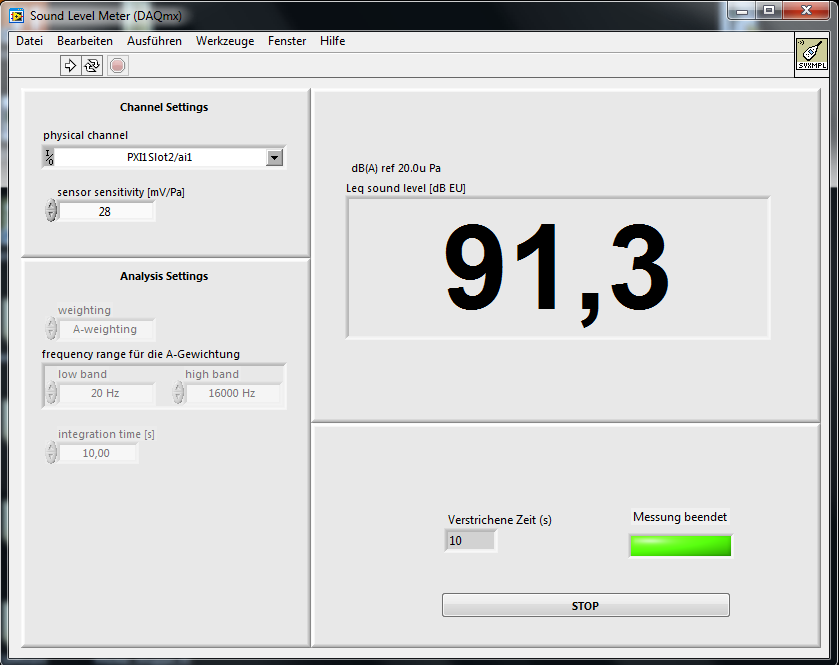
\includegraphics[width=0.7\textwidth]{pictures/Sound_level_meter.png}
	\caption{Frontpanel der Sound Level Meter VI}
	\label{fig:sound_level_meter}
\end{figure}

Die Abbildung \ref{fig:sound_level_meter} zeigt das Frontpanel der Sound Level Meter VI, zu erkennen ist die Mikrofonempfindlichkeit des iSEMcon Mikrofons und dass die Zeit der Mittelung auf \SI{10}{\second} gestellt ist. Rechts wird der gemittelte Wert angezeigt, welcher in diesem Testfall \SI{91,3}{\decibel} beträgt. 


\begin{figure}[H]
    \centering
    \begin{tikzpicture}
    \begin{polaraxis}[
        width=11cm, height=11cm,
        xtick={0,15,30,45,60,75,90,105,120,135,150,165,180,195,210,225,240,255,270,285,300,315,330,345},
        xticklabels={$0^\circ$,,$30^\circ$,,$60^\circ$,,$90^\circ$,,$120^\circ$,,$150^\circ$,,$180^\circ$,,$210^\circ$,,$240^\circ$,,$270^\circ$,,$300^\circ$,,$330^\circ$,},
        ytick={50,60,70,80},
        ymin=50, ymax=85,
        y coord trafo/.code={\pgfmathparse{#1}\pgfmathresult},
        y coord inv trafo/.code={\pgfmathparse{#1}\pgfmathresult},
        ylabel={$L_p$ [dB]},
        ylabel style={at={(0.5,1.08)}, font=\small},
        grid=both,
        grid style={line width=0.1pt, draw=gray!40},
        major grid style={line width=0.2pt, draw=gray!60},
        legend style={at={(1.3,1.0)}, anchor=north west, font=\scriptsize, fill=white, draw=gray},
        tick label style={font=\scriptsize},
    ]
    % SPL Messung 360
    \addplot[color=OBlue, thick] coordinates {
        (0,76.2)(15,77.9)(30,79.0)(45,78.4)(60,79.7)(75,74.8)(90,69.9)(105,77.7)(120,79.7)(135,78.5)(150,79.7)(165,79.2)(180,80.5)(195,79.9)(210,79.3)(225,78.6)(240,78.7)(255,75.5)(270,68.4)(285,78.3)(300,78.8)(315,78.1)(330,78.9)(345,78.6)(360,76.2)
    };
    \legend{SPL}
    \end{polaraxis}
    \end{tikzpicture}
    \caption{Horizontale Richtcharakteristik des DML-Lautsprechers -- SPL Messung}
    \label{fig:schallfeld_spl_messung}
\end{figure}

Abbildung~\ref{fig:schallfeld_spl_messung} zeigt die gemessene horizontale Richtcharakteristik des DML-Lautsprechers als Gesamtschalldruckpegel. Die Messwerte liegen im Bereich von \SI{68,4}{\decibel} bis \SI{80,5}{\decibel}, was einer Pegelschwankung von etwa \SI{12}{\decibel} entspricht. Das Abstrahlverhalten zeigt die für DML-Lautsprecher typische Dipolcharakteristik mit maximaler Abstrahlung in Richtung \SI{0}{\degree} zur Vorderseite und \SI{180}{\degree} an der Rückseite. Die minimalen Schalldruckpegel treten bei \SI{90}{\degree}, \SI{69,9}{\decibel} und \SI{270}{\degree}, \SI{68,4}{\decibel} auf, was auf die seitliche Auslöschung durch die gegenphasige Abstrahlung der Plattenvorder- und -rückseite zurückzuführen ist.



Die Richtcharakteristik wird zunächst als absoluter Schalldruckpegel und anschließend normiert auf die Hauptabstrahlrichtung (\SI{0}{\degree}) betrachtet, um sowohl das frequenzabhängige Abstrahlverhalten als auch die Richtwirkung des Lautsprechers zu beurteilen.


\begin{figure}[H]
    \centering
    \begin{tikzpicture}
    \begin{polaraxis}[
        width=11cm, height=11cm,
        xtick={0,30,60,90,120,150,180,210,240,270,300,330},
        xticklabels={$0^\circ$,$30^\circ$,$60^\circ$,$90^\circ$,$120^\circ$,$150^\circ$,$180^\circ$,$210^\circ$,$240^\circ$,$270^\circ$,$300^\circ$,$330^\circ$},
        ytick={20,30,40,50,60},
        ymin=20, ymax=65,
        y coord trafo/.code={\pgfmathparse{#1}\pgfmathresult},
        y coord inv trafo/.code={\pgfmathparse{#1}\pgfmathresult},
        ylabel={$L_p$ [dB]},
        ylabel style={at={(0.5,1.08)}, font=\small},
        grid=both,
        grid style={line width=0.1pt, draw=gray!40},
        major grid style={line width=0.2pt, draw=gray!60},
        legend style={at={(1.3,1.0)}, anchor=north west, font=\scriptsize, fill=white, draw=gray},
        tick label style={font=\scriptsize},
    ]
    % 63 Hz
    \addplot[color=OBlue, thick] coordinates {
        (0,37.6)(15,39.0)(30,37.9)(45,37.6)(60,34.1)(75,30.7)(90,30.3)(105,30.8)(120,32.5)(135,34.5)(150,36.2)(165,37.5)(180,37.4)(195,37.3)(210,36.7)(225,36.0)(240,35.6)(255,31.5)(270,31.0)(285,33.3)(300,35.2)(315,36.8)(330,36.6)(345,38.1)(360,37.6)
    };
    % 125 Hz
    \addplot[color=OBlue!70!black, thick, dashed] coordinates {
        (0,42.4)(15,41.7)(30,41.5)(45,39.4)(60,36.7)(75,32.8)(90,27.2)(105,30.5)(120,34.8)(135,37.7)(150,41.0)(165,41.0)(180,42.4)(195,42.5)(210,40.0)(225,39.9)(240,37.2)(255,31.8)(270,28.1)(285,35.3)(300,39.6)(315,41.4)(330,42.0)(345,42.4)(360,42.4)
    };
    % 250 Hz
    \addplot[color=OBlue!50, thick, dotted] coordinates {
        (0,44.2)(15,44.5)(30,44.2)(45,42.2)(60,40.0)(75,35.9)(90,29.4)(105,27.1)(120,33.8)(135,38.1)(150,40.7)(165,42.7)(180,44.9)(195,43.7)(210,42.4)(225,42.2)(240,39.9)(255,33.7)(270,24.3)(285,34.8)(300,39.8)(315,41.8)(330,42.4)(345,44.4)(360,44.2)
    };
    % 500 Hz
    \addplot[color=OOrange!70, thick] coordinates {
        (0,50.5)(15,50.7)(30,49.6)(45,48.2)(60,45.7)(75,41.5)(90,35.0)(105,36.6)(120,41.7)(135,44.3)(150,47.8)(165,49.1)(180,50.2)(195,49.5)(210,48.8)(225,48.2)(240,45.8)(255,40.0)(270,32.4)(285,38.7)(300,45.5)(315,48.2)(330,48.8)(345,49.8)(360,50.5)
    };
    % 1.000 Hz
    \addplot[color=OOrange, thick, dashed] coordinates {
        (0,54.8)(15,55.8)(30,55.5)(45,55.5)(60,52.9)(75,48.8)(90,38.3)(105,43.9)(120,49.5)(135,53.1)(150,54.7)(165,55.7)(180,54.5)(195,53.0)(210,52.7)(225,51.6)(240,50.8)(255,44.4)(270,34.4)(285,46.6)(300,52.3)(315,53.0)(330,53.8)(345,53.6)(360,54.8)
    };
    % 2.000 Hz
    \addplot[color=OOrange!50!red, thick, dotted] coordinates {
        (0,53.0)(15,52.1)(30,49.3)(45,47.2)(60,47.9)(75,47.0)(90,43.4)(105,36.7)(120,38.0)(135,42.4)(150,47.7)(165,49.9)(180,56.0)(195,54.3)(210,53.9)(225,53.6)(240,52.8)(255,48.2)(270,42.1)(285,45.5)(300,52.3)(315,51.0)(330,51.5)(345,54.0)(360,53.0)
    };
    % 4.000 Hz
    \addplot[color=gray!80, thick] coordinates {
        (0,59.4)(15,52.4)(30,55.1)(45,52.0)(60,43.9)(75,45.1)(90,43.6)(105,42.7)(120,40.7)(135,46.2)(150,52.6)(165,56.2)(180,58.4)(195,53.3)(210,49.4)(225,52.7)(240,57.7)(255,53.6)(270,40.1)(285,56.5)(300,58.0)(315,44.2)(330,44.2)(345,53.2)(360,59.4)
    };
    % 8.000 Hz
    \addplot[color=gray!60, thick, dashed] coordinates {
        (0,42.3)(15,44.0)(30,47.9)(45,49.5)(60,44.3)(75,49.1)(90,42.8)(105,42.1)(120,51.0)(135,53.0)(150,38.5)(165,41.8)(180,51.2)(195,49.9)(210,45.4)(225,45.8)(240,52.3)(255,46.6)(270,38.3)(285,49.4)(300,50.4)(315,46.0)(330,41.1)(345,45.7)(360,42.3)
    };
    % 16.000 Hz
    \addplot[color=gray!40, thick, dotted] coordinates {
        (0,37.9)(15,44.1)(30,32.0)(45,37.5)(60,33.4)(75,42.3)(90,38.0)(105,36.2)(120,33.7)(135,29.9)(150,34.2)(165,28.3)(180,33.4)(195,32.6)(210,29.9)(225,33.2)(240,44.1)(255,38.4)(270,31.1)(285,40.2)(300,44.1)(315,37.9)(330,36.6)(345,40.9)(360,37.9)
    };
    \legend{63 Hz, 125 Hz, 250 Hz, 500 Hz, 1 kHz, 2 kHz, 4 kHz, 8 kHz, 16 kHz}
    \end{polaraxis}
    \end{tikzpicture}
    \caption{Horizontale Richtcharakteristik des DML-Lautsprechers -- absoluter Schalldruckpegel $L_p$ [dB]}
    \label{fig:schallfeld_absolut}
\end{figure}

Abbildung~\ref{fig:schallfeld_absolut} zeigt die horizontale Richtcharakteristik des DML-Lautsprechers als absolute Schalldruckpegel. Im Tieftonbereich \SIrange{63}{125}{\hertz} sind die Pegel erwartungsgemäß niedrig und die Abstrahlung nahezu omnidirektional, da die Plattenabmessungen mit einer Plattendiagonale von ca.\ \SI{0{,}83}{\metre} von weit unterhalb der akustischen Wellenlänge bei \SI{125}{\hertz} $\lambda \approx \SI{2{,}7}{\metre}$ liegen.
 
Zwischen \SI{500}{\hertz} und \SI{2}{\kilo\hertz} steigen die abgestrahlten Pegel deutlich an und es formt sich die für DML-Lautsprecher typische Dipolcharakteristik mit Abstrahlung nach vorne und hinten. Die höchsten Absolutpegel treten bei ca.\ \SIrange{1}{2}{\kilo\hertz} auf, was auf den Bereich der Koinzidenzfrequenz hindeutet. Leichte Asymmetrien im Richtmuster sind auf die bewusst exzentrische Exciter-Positionierung zurückzuführen.
 
Im Hochtonbereich \SIrange{4}{16}{\kilo\hertz} fragmentiert das Abstrahlmuster zunehmend. Die Interferenz vieler gleichzeitig schwingender, phasenverschobener Plattenbereiche erzeugt zahlreiche Nebenkeulen und Einbrüche. Die bei diesen Frequenzen sichtbare Links-Rechts-Asymmetrie spiegelt die Exciter-Position wider, kann aber teilweise auch durch die manuelle Winkelpositionierung der Platte bedingt sein.



\begin{figure}[H]
    \centering
    \begin{tikzpicture}
    \begin{polaraxis}[
        width=11cm, height=11cm,
        xtick={0,30,60,90,120,150,180,210,240,270,300,330},
        xticklabels={$0^\circ$,$30^\circ$,$60^\circ$,$90^\circ$,$120^\circ$,$150^\circ$,$180^\circ$,$210^\circ$,$240^\circ$,$270^\circ$,$300^\circ$,$330^\circ$},
        ytick={-25,-20,-15,-10,-5,0,5,10},
        ymin=-25, ymax=15,
        y coord trafo/.code={\pgfmathparse{#1+25}\pgfmathresult},
        y coord inv trafo/.code={\pgfmathparse{#1-25}\pgfmathresult},
        ylabel={$\Delta L_p$ [dB]},
        ylabel style={at={(0.5,1.08)}, font=\small},
        grid=both,
        grid style={line width=0.1pt, draw=gray!40},
        major grid style={line width=0.2pt, draw=gray!60},
        legend style={at={(1.3,1.0)}, anchor=north west, font=\scriptsize, fill=white, draw=gray},
        tick label style={font=\scriptsize},
    ]
    % 63 Hz (normiert)
    \addplot[color=OBlue, thick] coordinates {
        (0,0.0)(15,1.4)(30,0.3)(45,-0.1)(60,-3.6)(75,-6.9)(90,-7.3)(105,-6.8)(120,-5.1)(135,-3.1)(150,-1.5)(165,-0.1)(180,-0.2)(195,-0.4)(210,-0.9)(225,-1.6)(240,-2.0)(255,-6.1)(270,-6.7)(285,-4.4)(300,-2.5)(315,-0.9)(330,-1.0)(345,0.5)(360,0.0)
    };
    % 125 Hz (normiert)
    \addplot[color=OBlue!70!black, thick, dashed] coordinates {
        (0,0.0)(15,-0.7)(30,-1.0)(45,-3.0)(60,-5.7)(75,-9.7)(90,-15.3)(105,-12.0)(120,-7.6)(135,-4.8)(150,-1.4)(165,-1.4)(180,-0.1)(195,0.1)(210,-2.4)(225,-2.5)(240,-5.3)(255,-10.6)(270,-14.4)(285,-7.1)(300,-2.9)(315,-1.1)(330,-0.4)(345,-0.1)(360,0.0)
    };
    % 250 Hz (normiert)
    \addplot[color=OBlue!50, thick, dotted] coordinates {
        (0,0.0)(15,0.3)(30,-0.1)(45,-2.0)(60,-4.2)(75,-8.3)(90,-14.8)(105,-17.1)(120,-10.5)(135,-6.1)(150,-3.5)(165,-1.5)(180,0.7)(195,-0.5)(210,-1.8)(225,-2.0)(240,-4.3)(255,-10.5)(270,-19.9)(285,-9.4)(300,-4.4)(315,-2.4)(330,-1.8)(345,0.2)(360,0.0)
    };
    % 500 Hz (normiert)
    \addplot[color=OOrange!70, thick] coordinates {
        (0,0.0)(15,0.2)(30,-0.8)(45,-2.3)(60,-4.8)(75,-9.0)(90,-15.5)(105,-13.9)(120,-8.8)(135,-6.2)(150,-2.7)(165,-1.4)(180,-0.2)(195,-1.0)(210,-1.7)(225,-2.3)(240,-4.7)(255,-10.4)(270,-18.1)(285,-11.8)(300,-5.0)(315,-2.3)(330,-1.7)(345,-0.7)(360,0.0)
    };
    % 1.000 Hz (normiert)
    \addplot[color=OOrange, thick, dashed] coordinates {
        (0,0.0)(15,1.0)(30,0.7)(45,0.7)(60,-2.0)(75,-6.1)(90,-16.5)(105,-11.0)(120,-5.4)(135,-1.7)(150,-0.1)(165,0.9)(180,-0.4)(195,-1.8)(210,-2.1)(225,-3.2)(240,-4.1)(255,-10.5)(270,-20.4)(285,-8.3)(300,-2.6)(315,-1.8)(330,-1.0)(345,-1.2)(360,0.0)
    };
    % 2.000 Hz (normiert)
    \addplot[color=OOrange!50!red, thick, dotted] coordinates {
        (0,0.0)(15,-0.9)(30,-3.7)(45,-5.8)(60,-5.1)(75,-5.9)(90,-9.5)(105,-16.3)(120,-15.0)(135,-10.6)(150,-5.3)(165,-3.1)(180,3.0)(195,1.4)(210,0.9)(225,0.6)(240,-0.2)(255,-4.8)(270,-10.9)(285,-7.4)(300,-0.7)(315,-2.0)(330,-1.5)(345,1.0)(360,0.0)
    };
    % 4.000 Hz (normiert)
    \addplot[color=gray!80, thick] coordinates {
        (0,0.0)(15,-7.0)(30,-4.3)(45,-7.4)(60,-15.5)(75,-14.3)(90,-15.8)(105,-16.7)(120,-18.7)(135,-13.2)(150,-6.9)(165,-3.2)(180,-1.0)(195,-6.1)(210,-10.0)(225,-6.8)(240,-1.7)(255,-5.9)(270,-19.3)(285,-2.9)(300,-1.4)(315,-15.2)(330,-15.2)(345,-6.2)(360,0.0)
    };
    % 8.000 Hz (normiert)
    \addplot[color=gray!60, thick, dashed] coordinates {
        (0,0.0)(15,1.7)(30,5.6)(45,7.2)(60,2.0)(75,6.8)(90,0.5)(105,-0.2)(120,8.7)(135,10.7)(150,-3.8)(165,-0.5)(180,8.9)(195,7.6)(210,3.1)(225,3.5)(240,10.0)(255,4.3)(270,-3.9)(285,7.1)(300,8.2)(315,3.7)(330,-1.2)(345,3.4)(360,0.0)
    };
    % 16.000 Hz (normiert)
    \addplot[color=gray!40, thick, dotted] coordinates {
        (0,0.0)(15,6.2)(30,-5.8)(45,-0.4)(60,-4.5)(75,4.5)(90,0.2)(105,-1.7)(120,-4.1)(135,-8.0)(150,-3.6)(165,-9.5)(180,-4.5)(195,-5.2)(210,-8.0)(225,-4.6)(240,6.3)(255,0.6)(270,-6.7)(285,2.3)(300,6.3)(315,0.1)(330,-1.3)(345,3.0)(360,0.0)
    };
    \legend{63 Hz, 125 Hz, 250 Hz, 500 Hz, 1 kHz, 2 kHz, 4 kHz, 8 kHz, 16 kHz}
    \end{polaraxis}
    \end{tikzpicture}
    \caption{Horizontale Richtcharakteristik des DML-Lautsprechers -- auf $0^\circ$ normierter Schalldruckpegel $\Delta L_p$ [dB]}
    \label{fig:schallfeld_normiert}
\end{figure}


Die auf \SI{0}{\degree} normierte Darstellung in Abbildung~\ref{fig:schallfeld_normiert} isoliert die frequenzabhängige Richtwirkung von den absoluten Pegelunterschieden. Bei \SIrange{63}{125}{\hertz} weicht der Pegel über alle Winkel um weniger als ca.\ \SI{5}{\deci\bel} ab -- die Abstrahlung ist nahezu kreisförmig.
 
Zwischen \SI{250}{\hertz} und \SI{1}{\kilo\hertz} bildet sich eine ausgeprägte Dipolform mit Einbrüchen von \SIrange{15}{25}{\deci\bel} bei \SI{90}{\degree} und \SI{270}{\degree}. Die Nullstellen sind erwartungsgemäß weniger scharf als bei einem idealen Punktdipol, da die Platte einen ausgedehnten Strahler mit endlicher Fläche und Kantenbeugung darstellt.
 
Ab \SI{2}{\kilo\hertz} verengt sich die Hauptkeule und es entstehen zunehmend Nebenkeulen. Bei \SI{8}{\kilo\hertz} und \SI{16}{\kilo\hertz} ist das Richtmuster stark fragmentiert. Die Winkelauflösung von \SI{15}{\degree} reicht in diesem Frequenzbereich möglicherweise nicht aus, um alle schmalen Keulen und Nullstellen vollständig aufzulösen.


\clearpage

Bei der Frequenzgangmessung wurde zur Vergleichbarkeit ein konventioneller Kolbenstrahllautsprecher der Firma Bose als Referenz herangezogen. Dabei handelt es sich um das Modell Bose ML3 BLK (Artikelnummer 125727), einen kompakten Fullrange-Lautsprecher.

\begin{figure}[H]
	\centering
	\includegraphics[width=0.6\textwidth]{pictures/Bose_Referenz.png}
	\caption{Bose ML3 BLK Referenzlautsprecher}
	\label{fig:bose_referenz}
\end{figure}

Abbildung \ref{fig:bose_referenz} zeigt den Bose ML3 BLK Lautsprecher, welcher als Fullrange-System mit Hoch-, Mittel- und Tieftöner ausgestattet ist. Der Vergleich mit einem konventionellen Kolbenstrahler ermöglicht eine Einordnung der DML-Lautsprecher hinsichtlich Frequenzgang und Abstrahlverhalten. 


Zum Vermessen der Lautsprecher wurde das in Kapitel 3.4.2 beschriebene LabVIEW VI verwendet. 


\begin{figure}[H]
	\centering
	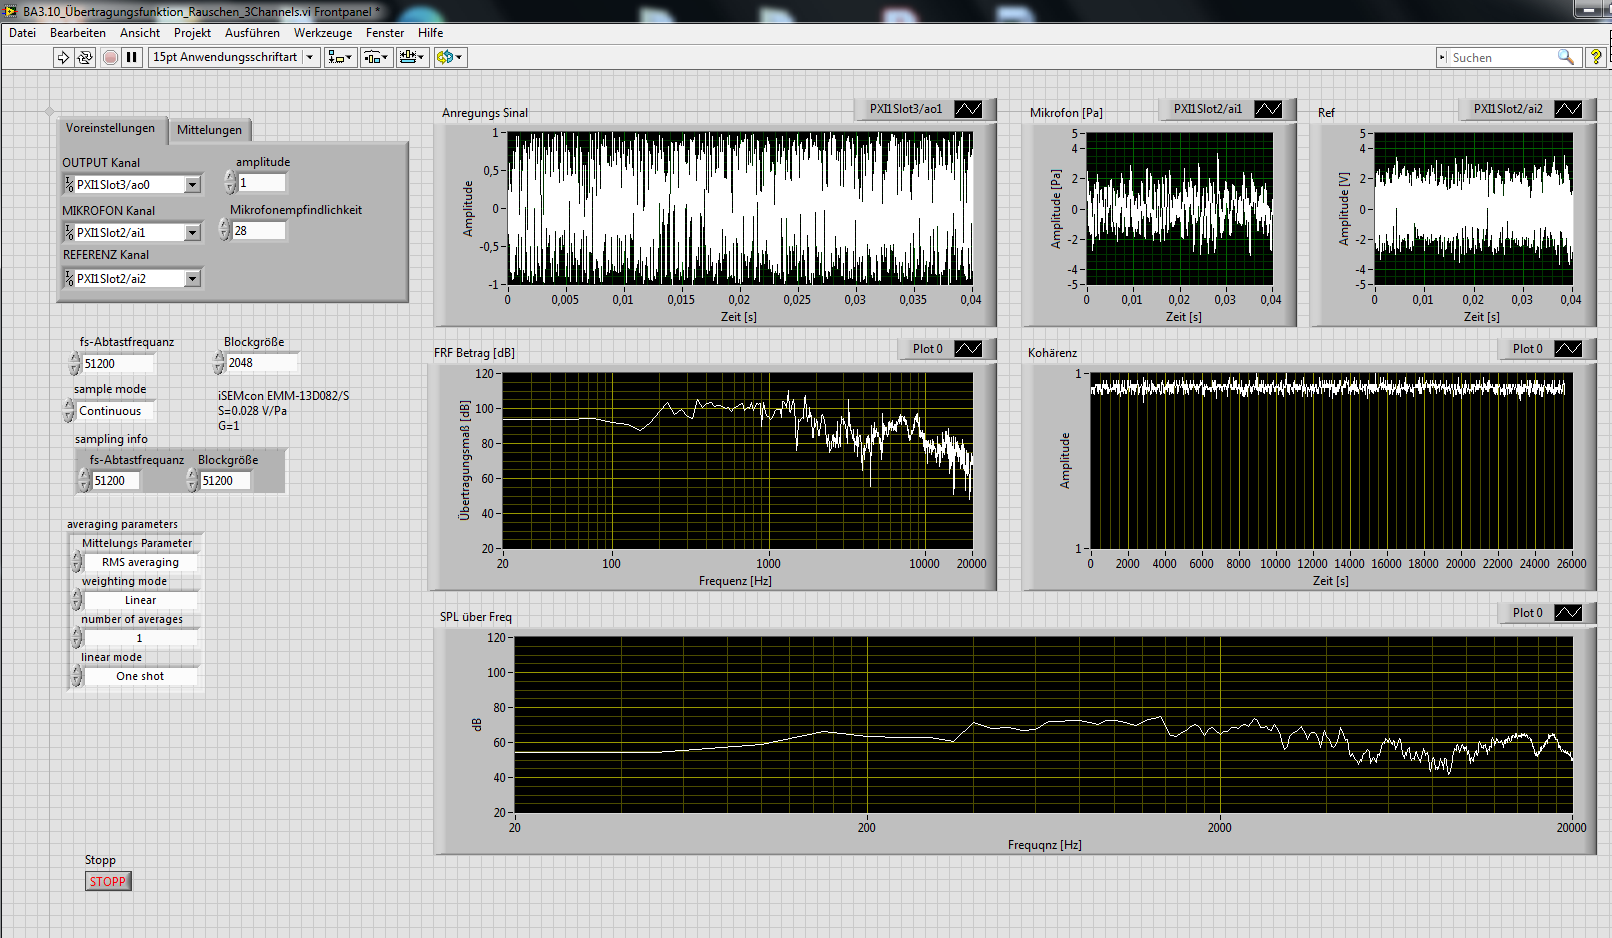
\includegraphics[width=0.8\textwidth]{pictures/Frontpanel.png}
	\caption{Frontpanel des LabVIEW VI während einer Messung}
	\label{fig:frontpanel_labview}
\end{figure}

In Abbildung \ref{fig:frontpanel_labview} wird das Frontpanel während einer Messung gezeigt, zu erkennen ist die Anregung mittels weißem Rauschen im Graphen oben links. Das Mikrofon- und Referenzsignal werden oben rechts angezeigt. In der Mitte des Frontpanels wird die FRF-Übertragungsfunktion und die zugehörige Kohärenz graphisch dargestellt. Unten wird der Schalldruckpegel über der Frequenz dargestellt. 


\begin{figure}[H]
    \centering
    \begin{tikzpicture}
    \begin{semilogxaxis}[
        width=14cm, height=9cm,
        xlabel={Frequenz $f$ [Hz]},
        ylabel={Schalldruckpegel $L_p$ [dB]},
        xmin=20, xmax=20000,
        ymin=0, ymax=120,
        xtick={100, 1000, 10000},
        xticklabels={100, 1.000, 10.000},
        minor xtick={20,30,40,50,60,70,80,90,200,300,400,500,600,700,800,900,2000,3000,4000,5000,6000,7000,8000,9000,20000},
        ytick={0,20,40,60,80,100,120},
        grid=both,
        grid style={line width=0.1pt, draw=gray!30},
        major grid style={line width=0.2pt, draw=gray!50},
        legend style={at={(0.02,0.02)}, anchor=south west, font=\footnotesize, fill=white, fill opacity=0.8, draw=gray},
        tick label style={font=\small},
        label style={font=\small},
    ]
    % 70x44 Hersteller
    \addplot[color=OBlue, thick] coordinates {
        (25,98.5) (150,82.9) (275,97.4) (400,97.9) (525,98.8) (650,94.6) (775,86.5) (900,92.5) (1025,92.7) (1150,90.2) (1275,88.2) (1400,88.6) (1525,88.8) (1650,94.0) (1775,94.4) (1900,78.8) (2025,87.7) (2150,87.3) (2275,89.1) (2400,81.2) (2525,89.5) (2650,78.2) (2775,81.9) (2900,81.4) (3025,87.1) (3150,88.2) (3275,88.5) (3400,82.2) (3525,81.2) (3650,71.4) (3775,81.0) (3900,74.9) (4025,83.2) (4150,84.8) (4275,76.8) (4400,82.9) (4525,75.4) (4650,71.3) (4775,68.7) (4900,74.8) (5025,79.2) (5150,84.4) (5275,75.9) (5400,79.6) (5525,81.3) (5650,76.2) (5775,84.1) (5900,85.7) (6025,77.2) (6150,78.3) (6275,86.7) (6400,77.7) (6525,79.1) (6650,78.0) (6775,75.5) (6900,80.3) (7025,79.3) (7150,81.4) (7275,84.5) (7400,88.2) (7525,86.8) (7650,89.3) (7775,86.5) (7900,84.3) (8025,86.3) (8150,79.3) (8275,74.8) (8400,79.9) (8525,82.9) (8650,80.6) (8775,90.9) (8900,80.3) (9025,79.6) (9150,80.0) (9275,82.9) (9400,83.1) (9525,78.8) (9650,82.9) (9775,80.5) (9900,83.0) (10025,72.8) (10150,83.0) (10275,76.3) (10400,74.7) (10525,74.7) (10650,76.5) (10775,74.2) (10900,73.4) (11025,73.1) (11150,76.7) (11275,73.0) (11400,74.8) (11525,74.7) (11650,72.1) (11775,71.8) (11900,73.8) (12025,73.6) (12150,71.9) (12275,74.9) (12400,58.1) (12525,69.3) (12650,62.8) (12775,61.8) (12900,57.7) (13025,67.0) (13150,56.9) (13275,68.5) (13400,66.1) (13525,64.6) (13650,70.1) (13775,77.6) (13900,70.3) (14025,75.7) (14150,76.4) (14275,71.4) (14400,69.2) (14525,66.6) (14650,76.5) (14775,63.1) (14900,70.5) (15025,66.8) (15150,73.1) (15275,70.2) (15400,66.6) (15525,72.4) (15650,71.0) (15775,69.1) (15900,72.4) (16025,70.0) (16150,68.6) (16275,69.5) (16400,59.9) (16525,67.6) (16650,64.8) (16775,72.2) (16900,75.8) (17025,63.7) (17150,67.2) (17275,70.9) (17400,70.9) (17525,72.2) (17650,72.1) (17775,75.5) (17900,68.2) (18025,62.3) (18150,65.7) (18275,72.9) (18400,76.2) (18525,64.7) (18650,63.8) (18775,68.3) (18900,68.6) (19025,68.1) (19150,73.2) (19275,73.3) (19400,77.6) (19525,77.0) (19650,72.8) (19775,76.3) (19900,78.9)
    };
    % 70x44 Skript
    \addplot[color=OOrange, thick] coordinates {
        (25,91.0) (150,81.7) (275,88.2) (400,96.0) (525,95.6) (650,94.4) (775,85.0) (900,84.7) (1025,89.8) (1150,89.4) (1275,97.7) (1400,97.1) (1525,88.3) (1650,89.4) (1775,90.4) (1900,87.6) (2025,89.6) (2150,90.0) (2275,87.4) (2400,88.2) (2525,71.9) (2650,77.8) (2775,74.6) (2900,80.9) (3025,77.3) (3150,88.4) (3275,87.6) (3400,82.8) (3525,84.7) (3650,79.9) (3775,75.4) (3900,81.4) (4025,84.2) (4150,77.6) (4275,75.4) (4400,75.1) (4525,76.8) (4650,62.1) (4775,76.1) (4900,88.4) (5025,75.0) (5150,75.8) (5275,76.3) (5400,68.3) (5525,74.9) (5650,81.6) (5775,73.4) (5900,83.3) (6025,81.1) (6150,78.1) (6275,75.7) (6400,83.5) (6525,78.4) (6650,79.2) (6775,80.2) (6900,79.8) (7025,84.5) (7150,82.2) (7275,90.0) (7400,88.1) (7525,82.0) (7650,89.0) (7775,79.3) (7900,78.0) (8025,76.1) (8150,72.5) (8275,69.4) (8400,81.9) (8525,75.7) (8650,82.1) (8775,79.6) (8900,73.5) (9025,81.7) (9150,79.8) (9275,74.8) (9400,81.6) (9525,72.0) (9650,70.6) (9775,77.0) (9900,73.8) (10025,73.9) (10150,75.1) (10275,73.9) (10400,75.7) (10525,66.3) (10650,72.1) (10775,67.2) (10900,79.1) (11025,59.8) (11150,69.3) (11275,71.4) (11400,68.5) (11525,65.0) (11650,71.4) (11775,61.8) (11900,66.9) (12025,68.6) (12150,61.3) (12275,64.2) (12400,64.2) (12525,72.3) (12650,61.0) (12775,61.8) (12900,71.4) (13025,64.0) (13150,65.3) (13275,63.5) (13400,68.2) (13525,72.8) (13650,65.5) (13775,66.1) (13900,64.6) (14025,77.3) (14150,70.7) (14275,66.9) (14400,71.5) (14525,67.4) (14650,71.6) (14775,70.6) (14900,70.9) (15025,75.4) (15150,73.4) (15275,75.4) (15400,71.5) (15525,72.5) (15650,80.0) (15775,76.3) (15900,73.7) (16025,79.0) (16150,75.1) (16275,77.5) (16400,81.2) (16525,76.3) (16650,76.3) (16775,80.4) (16900,72.4) (17025,76.4) (17150,78.8) (17275,71.6) (17400,77.8) (17525,78.3) (17650,72.2) (17775,75.8) (17900,70.6) (18025,69.9) (18150,75.2) (18275,78.5) (18400,73.8) (18525,75.4) (18650,75.2) (18775,81.3) (18900,76.5) (19025,69.9) (19150,69.0) (19275,70.5) (19400,67.5) (19525,72.0) (19650,76.4) (19775,73.2) (19900,75.4)
    };
    % 100x70 Hersteller
    \addplot[color=OBlue, thick, dashed] coordinates {
        (25,91.6) (150,92.8) (275,93.0) (400,96.6) (525,90.5) (650,91.2) (775,91.9) (900,89.8) (1025,97.1) (1150,88.5) (1275,98.1) (1400,92.4) (1525,89.4) (1650,88.3) (1775,86.6) (1900,80.3) (2025,80.6) (2150,91.3) (2275,82.1) (2400,74.3) (2525,74.6) (2650,73.6) (2775,75.1) (2900,74.4) (3025,77.4) (3150,86.8) (3275,85.6) (3400,85.9) (3525,83.4) (3650,79.5) (3775,75.4) (3900,85.0) (4025,75.3) (4150,76.0) (4275,81.5) (4400,72.3) (4525,67.9) (4650,72.5) (4775,84.8) (4900,77.5) (5025,77.1) (5150,84.0) (5275,79.0) (5400,81.8) (5525,86.5) (5650,82.5) (5775,71.8) (5900,83.4) (6025,83.0) (6150,79.9) (6275,85.4) (6400,76.6) (6525,77.5) (6650,76.0) (6775,82.5) (6900,78.9) (7025,85.8) (7150,87.0) (7275,86.5) (7400,81.9) (7525,79.4) (7650,81.6) (7775,76.6) (7900,70.2) (8025,67.8) (8150,72.7) (8275,80.7) (8400,79.5) (8525,81.8) (8650,86.4) (8775,82.0) (8900,80.2) (9025,73.3) (9150,73.7) (9275,75.0) (9400,62.8) (9525,75.4) (9650,74.4) (9775,70.7) (9900,72.8) (10025,68.4) (10150,67.4) (10275,68.2) (10400,62.6) (10525,67.1) (10650,71.5) (10775,58.2) (10900,67.6) (11025,58.7) (11150,67.7) (11275,71.4) (11400,65.1) (11525,73.7) (11650,69.4) (11775,65.7) (11900,61.8) (12025,74.6) (12150,63.8) (12275,64.7) (12400,64.7) (12525,61.8) (12650,63.0) (12775,69.8) (12900,70.7) (13025,65.6) (13150,68.4) (13275,72.4) (13400,68.0) (13525,72.8) (13650,75.4) (13775,73.1) (13900,74.1) (14025,82.4) (14150,74.9) (14275,75.6) (14400,75.3) (14525,76.7) (14650,75.2) (14775,80.3) (14900,78.2) (15025,75.2) (15150,72.4) (15275,75.9) (15400,72.1) (15525,75.1) (15650,78.9) (15775,71.0) (15900,77.0) (16025,78.5) (16150,71.1) (16275,78.0) (16400,72.7) (16525,75.6) (16650,76.6) (16775,77.3) (16900,77.8) (17025,76.7) (17150,79.2) (17275,77.4) (17400,78.6) (17525,73.9) (17650,75.5) (17775,78.3) (17900,74.0) (18025,78.2) (18150,79.3) (18275,80.3) (18400,78.0) (18525,79.6) (18650,81.5) (18775,78.5) (18900,79.1) (19025,84.2) (19150,81.6) (19275,80.5) (19400,80.4) (19525,79.8) (19650,77.1) (19775,80.4) (19900,80.3)
    };
    % 100x70 Skript
    \addplot[color=OOrange, thick, dashed] coordinates {
        (25,89.9) (150,90.0) (275,90.8) (400,90.2) (525,93.3) (650,83.3) (775,91.0) (900,84.4) (1025,89.5) (1150,94.2) (1275,93.5) (1400,84.0) (1525,83.5) (1650,78.8) (1775,66.9) (1900,88.8) (2025,81.4) (2150,76.8) (2275,91.0) (2400,85.8) (2525,86.1) (2650,89.6) (2775,75.0) (2900,83.6) (3025,70.1) (3150,86.1) (3275,88.6) (3400,85.0) (3525,75.7) (3650,73.8) (3775,82.5) (3900,75.7) (4025,80.5) (4150,79.9) (4275,67.9) (4400,65.1) (4525,75.1) (4650,78.9) (4775,70.9) (4900,73.4) (5025,75.9) (5150,80.2) (5275,66.6) (5400,83.6) (5525,90.8) (5650,69.1) (5775,80.2) (5900,80.1) (6025,84.3) (6150,83.5) (6275,87.8) (6400,87.1) (6525,86.8) (6650,83.8) (6775,89.4) (6900,85.4) (7025,92.2) (7150,90.8) (7275,89.9) (7400,83.8) (7525,77.5) (7650,71.6) (7775,59.7) (7900,68.8) (8025,73.4) (8150,78.9) (8275,79.4) (8400,81.6) (8525,79.9) (8650,82.9) (8775,69.5) (8900,83.2) (9025,72.2) (9150,83.6) (9275,71.8) (9400,77.1) (9525,80.1) (9650,79.3) (9775,75.0) (9900,81.0) (10025,80.4) (10150,78.2) (10275,80.2) (10400,80.2) (10525,77.7) (10650,77.8) (10775,79.9) (10900,74.3) (11025,76.1) (11150,77.7) (11275,76.9) (11400,78.1) (11525,76.6) (11650,72.7) (11775,78.3) (11900,75.7) (12025,76.4) (12150,70.6) (12275,71.0) (12400,72.0) (12525,75.4) (12650,67.6) (12775,70.9) (12900,71.4) (13025,63.4) (13150,78.2) (13275,65.2) (13400,75.8) (13525,63.7) (13650,77.6) (13775,77.5) (13900,74.3) (14025,71.0) (14150,77.5) (14275,62.2) (14400,67.8) (14525,81.4) (14650,74.3) (14775,67.3) (14900,66.1) (15025,73.2) (15150,69.0) (15275,71.4) (15400,68.5) (15525,72.5) (15650,67.7) (15775,68.4) (15900,61.5) (16025,68.0) (16150,75.1) (16275,72.3) (16400,70.3) (16525,70.5) (16650,76.5) (16775,75.5) (16900,68.2) (17025,72.1) (17150,75.6) (17275,71.0) (17400,75.2) (17525,66.4) (17650,73.3) (17775,62.8) (17900,67.0) (18025,61.1) (18150,75.9) (18275,64.3) (18400,68.9) (18525,70.0) (18650,67.5) (18775,66.3) (18900,66.7) (19025,72.4) (19150,71.7) (19275,74.7) (19400,71.9) (19525,77.7) (19650,69.6) (19775,68.5) (19900,65.6)
    };
    % Bose Referenz
    \addplot[color=gray, thick, dotted] coordinates {
        (25,93.5) (150,86.8) (275,88.6) (400,86.5) (525,85.0) (650,85.6) (775,85.4) (900,88.1) (1025,84.2) (1150,87.0) (1275,85.2) (1400,84.3) (1525,82.8) (1650,72.0) (1775,77.9) (1900,81.4) (2025,77.0) (2150,65.8) (2275,63.8) (2400,65.4) (2525,58.0) (2650,63.7) (2775,64.2) (2900,51.5) (3025,69.2) (3150,73.1) (3275,73.0) (3400,73.6) (3525,79.6) (3650,78.2) (3775,77.4) (3900,78.9) (4025,73.7) (4150,83.0) (4275,80.0) (4400,77.3) (4525,76.3) (4650,89.1) (4775,80.6) (4900,77.4) (5025,81.3) (5150,78.2) (5275,87.6) (5400,76.2) (5525,76.2) (5650,74.9) (5775,71.0) (5900,71.4) (6025,79.3) (6150,69.1) (6275,67.9) (6400,66.8) (6525,64.0) (6650,67.1) (6775,61.7) (6900,62.4) (7025,60.6) (7150,63.5) (7275,71.8) (7400,60.8) (7525,59.7) (7650,51.6) (7775,55.7) (7900,61.8) (8025,57.1) (8150,59.5) (8275,56.8) (8400,60.4) (8525,54.1) (8650,54.6) (8775,56.9) (8900,55.6) (9025,66.2) (9150,55.3) (9275,55.4) (9400,56.7) (9525,57.4) (9650,63.2) (9775,69.1) (9900,61.8) (10025,63.2) (10150,54.1) (10275,58.9) (10400,52.2) (10525,54.0) (10650,56.7) (10775,62.4) (10900,56.3) (11025,56.7) (11150,57.5) (11275,58.4) (11400,55.9) (11525,60.0) (11650,50.1) (11775,58.7) (11900,53.7) (12025,56.4) (12150,53.4) (12275,49.4) (12400,52.4) (12525,48.1) (12650,47.1) (12775,42.0) (12900,47.7) (13025,45.8) (13150,43.6) (13275,42.0) (13400,38.3) (13525,49.9) (13650,40.4) (13775,55.2) (13900,46.7) (14025,40.7) (14150,42.7) (14275,45.1) (14400,43.0) (14525,43.0) (14650,44.9) (14775,46.6) (14900,47.0) (15025,46.1) (15150,42.7) (15275,45.6) (15400,51.7) (15525,45.6) (15650,43.2) (15775,41.4) (15900,44.6) (16025,52.4) (16150,47.7) (16275,42.4) (16400,47.7) (16525,47.2) (16650,38.1) (16775,39.9) (16900,43.2) (17025,38.0) (17150,41.5) (17275,40.3) (17400,37.3) (17525,40.2) (17650,42.6) (17775,41.1) (17900,44.6) (18025,38.8) (18150,44.9) (18275,44.5) (18400,48.1) (18525,41.5) (18650,45.5) (18775,49.5) (18900,46.0) (19025,51.6) (19150,44.9) (19275,46.9) (19400,46.5) (19525,46.4) (19650,50.0) (19775,47.6) (19900,51.5)
    };
    \legend{70$\times$44 Hersteller, 70$\times$44 Skript, 100$\times$70 Hersteller, 100$\times$70 Skript, Bose Referenz}
    \end{semilogxaxis}
    \end{tikzpicture}
    \caption{FRF Übertragungsfunktion -- Vergleich aller Messungen}
    \label{fig:frequenzgang_vergleich}
\end{figure}

Abbildung \ref{fig:frequenzgang_vergleich} zeigt die FRF-Übertragungsfunktionen (Frequency Response Function) beider DML-Platten im direkten Vergleich. Die FRF beschreibt das Verhältnis zwischen Ausgangs- und Eingangssignal eines Systems im Frequenzbereich und ermöglicht somit eine Aussage über das frequenzabhängige Übertragungsverhalten. Die Gültigkeit dieser Messungen wird durch die in Abbildung \ref{fig:kohaerenz_vergleich} dargestellte Kohärenz bestätigt, welche während der Messungen durchgehend bei ca.\,0{,}9 bis nahe 1 lag. Eine hohe Kohärenz bedeutet, dass das gemessene Ausgangssignal kausal mit dem Eingangssignal zusammenhängt und die Messung somit zuverlässig ist. Im Graphen ist zu erkennen, dass die 70$\times$44\,cm Platte mit der Hersteller-Position (dunkelblau, durchgezogen) im Tieftonbereich einen deutlichen Einbruch von ca.\,25\,dB bei etwa 80\,Hz aufweist, während die Skript-Position (orange, durchgezogen) einen deutlich gleichmäßigeren Verlauf zeigt. Die 100$\times$70\,cm Platte (gestrichelte Linien) weist generell einen stabileren Tieftonbereich auf, zeigt aber im Mittel- und Hochtonbereich stärkere Schwankungen. Die Bose-Referenz (grau, gepunktet) fällt oberhalb von 2\,kHz stark ab und ist den DML-Varianten im Hochtonbereich deutlich unterlegen.

Für die vorliegende Arbeit wird das DML-System mit den Abmessungen 70×44 cm gewählt. Diese Entscheidung stützt sich auf mehrere Faktoren, die sowohl die praktische Handhabbarkeit als auch die wissenschaftliche Aussagekraft der Untersuchung betreffen.
Ein wesentlicher Vorteil des kleineren Formats liegt in seiner Kompaktheit und Integrierbarkeit. Mit 70×44 cm lässt sich das Panel deutlich einfacher in reale Anwendungsszenarien einbinden als die größere 100×70 cm Variante – sei es als Wandelement, Deckenpaneel oder als in Möbel integrierte Schallquelle. Insbesondere in Kontexten wie Smart-Home-Umgebungen, Büroräumen oder Fahrzeuginnenräumen erweist sich die kompaktere Bauform als entscheidender Praxisvorteil, während eine Platte von 100×70 cm in vielen dieser Szenarien schlicht zu groß wäre.


Darüber hinaus zeigt die skriptbasierte Exciter-Positionierung gerade bei der 70×44 cm Platte ihre Stärken besonders überzeugend. Der Frequenzgang verläuft über den gesamten Übertragungsbereich deutlich glatter als bei der Herstellerposition, und im Gegensatz zur 100×70 cm Platte, bei der die Skript-Position im Tiefton eine Schwäche aufweist, funktioniert die rechnerisch optimierte Positionierung bei der kleineren Platte konsistent gut. Dieser Umstand bestätigt die Anwendbarkeit der zugrunde liegenden Simulationsmethodik und liefert damit einen wissenschaftlich verwertbaren Beitrag.
Auch messtechnisch bietet die kleinere Platte Vorteile. Die Messergebnisse zeigen einen klar erkennbaren Unterschied zwischen Hersteller- und Skript-Position: Während die Herstellerposition einen markanten Einbruch von rund 25 dB bei etwa 80 Hz aufweist, vermeidet die Skript-Position dieses Problem vollständig. Bei der 100×70 cm Platte fallen die Unterschiede zwischen beiden Positionen deutlich geringer aus. Die stärkere Differenzierbarkeit bei der kleineren Platte ermöglicht somit eine aussagekräftigere Bewertung der Positionierungsstrategien und stärkt die Argumentation der Arbeit.


Hinzu kommt, dass die kleinere Platte im Versuchsaufbau leichter zu handhaben ist. Ihr geringeres Gewicht erleichtert sowohl das Aufhängen im Freifeldraum als auch den Wechsel der Exciter-Positionen zwischen den einzelnen Messreihen. Dies reduziert systematische Fehlerquellen und erhöht die Reproduzierbarkeit der Ergebnisse – ein nicht zu unterschätzender Faktor, wenn mehrere Konfigurationen miteinander verglichen werden sollen.


Bezüglich der Fullrange-Tauglichkeit ist die 70×44 cm Platte mit der Skript-Position in Kombination mit einem Equalizer durchaus als breitbandiges Wiedergabesystem einsetzbar. Der gleichmäßige Frequenzgangverlauf ab ca. 60 Hz mit Pegeln von 87–92 dB stellt eine solide Ausgangsbasis dar, die sich mit moderatem EQ-Eingriff zu einem ausgewogenen System formen lässt. Der im Vergleich zur größeren Platte naturgemäß geringere Tieftonpegel unterhalb von 80 Hz wird in vielen praktischen Anwendungen ohnehin durch raumakustische Verstärkungseffekte oder einen ergänzenden Subwoofer kompensiert.


\begin{figure}[H]
    \centering
    \begin{tikzpicture}
    \begin{semilogxaxis}[
        width=14cm, height=9cm,
        xlabel={Frequenz $f$ [Hz]},
        ylabel={Schalldruckpegel $L_p$ [dB]},
        xmin=20, xmax=20000,
        ymin=15, ymax=70,
        xtick={100, 1000, 10000},
        xticklabels={100, 1.000, 10.000},
        minor xtick={20,30,40,50,60,70,80,90,200,300,400,500,600,700,800,900,2000,3000,4000,5000,6000,7000,8000,9000,20000},
        ytick={20,30,40,50,60,70},
        grid=both,
        grid style={line width=0.1pt, draw=gray!30},
        major grid style={line width=0.2pt, draw=gray!50},
        legend style={at={(0.02,0.02)}, anchor=south west, font=\small, fill=white, fill opacity=0.8, draw=gray},
        tick label style={font=\small},
        label style={font=\small},
    ]
    % Hersteller-Position (70x44)
    \addplot[color=OBlue, thick] coordinates {
        (25,40.0) (50,41.2) (100,41.4) (150,48.3) (200,46.9) (250,45.5) (300,46.5) (350,45.2) (400,54.3) (450,53.7) (500,52.5) (550,52.9) (600,53.1) (650,55.7) (700,57.5) (750,57.9) (800,57.9) (850,56.4) (900,57.1) (950,57.5) (1000,56.6) (1050,55.8) (1100,55.2) (1150,56.3) (1200,56.1) (1250,57.3) (1300,56.6) (1350,57.7) (1400,59.2) (1450,54.7) (1500,50.9) (1550,52.1) (1600,48.3) (1650,51.6) (1700,50.2) (1750,53.4) (1800,54.3) (1850,53.7) (1900,53.1) (1950,52.0) (2000,52.6) (2050,54.3) (2100,50.4) (2150,50.5) (2200,52.2) (2250,54.1) (2300,51.1) (2350,52.8) (2400,56.3) (2450,57.1) (2500,56.4) (2550,52.1) (2600,51.6) (2650,50.8) (2700,53.9) (2750,54.4) (2800,53.2) (2850,54.4) (2900,53.9) (2950,53.6) (3000,54.1) (3050,55.8) (3100,55.8) (3150,56.8) (3200,55.7) (3250,55.8) (3300,56.9) (3350,55.3) (3400,50.9) (3450,48.5) (3500,51.9) (3550,56.1) (3600,51.8) (3650,44.4) (3700,49.2) (3750,48.4) (3800,44.5) (3850,45.3) (3900,48.4) (3950,51.3) (4000,51.9) (4050,52.2) (4100,51.1) (4150,46.4) (4200,47.4) (4250,47.8) (4300,47.2) (4350,44.5) (4400,47.5) (4450,48.5) (4500,44.6) (4550,49.1) (4600,53.0) (4650,51.1) (4700,51.8) (4750,51.9) (4800,46.5) (4850,49.8) (4900,50.0) (4950,48.4) (5000,46.1) (5050,47.7) (5100,46.2) (5150,41.9) (5200,41.2) (5250,42.5) (5300,42.4) (5350,42.8) (5400,40.7) (5450,40.4) (5500,41.0) (5550,42.7) (5600,42.9) (5650,42.8) (5700,38.5) (5750,39.5) (5800,42.7) (5850,38.8) (5900,42.2) (5950,43.4) (6000,48.9) (6050,48.2) (6100,44.9) (6150,42.5) (6200,45.0) (6250,45.0) (6300,50.3) (6350,50.8) (6400,51.5) (6450,50.6) (6500,48.8) (6550,49.0) (6600,47.5) (6650,49.8) (6700,47.4) (6750,47.1) (6800,47.4) (6850,47.8) (6900,48.2) (6950,48.0) (7000,42.7) (7050,40.6) (7100,37.9) (7150,42.7) (7200,42.2) (7250,36.2) (7300,36.6) (7350,38.0) (7400,35.6) (7450,38.4) (7500,36.9) (7550,40.9) (7600,43.4) (7650,41.2) (7700,38.9) (7750,36.7) (7800,37.6) (7850,42.6) (7900,43.5) (7950,45.6) (8000,46.6) (8050,44.6) (8100,43.3) (8150,41.5) (8200,40.6) (8250,43.6) (8300,47.5) (8350,50.1) (8400,49.0) (8450,46.4) (8500,44.0) (8550,38.5) (8600,40.4) (8650,42.6) (8700,43.4) (8750,44.7) (8800,44.1) (8850,42.3) (8900,39.3) (8950,36.7) (9000,34.5) (9050,41.3) (9100,43.9) (9150,43.6) (9200,38.7) (9250,34.2) (9300,36.8) (9350,37.1) (9400,36.6) (9450,36.9) (9500,41.3) (9550,41.7) (9600,39.8) (9650,38.2) (9700,37.4) (9750,34.7) (9800,39.4) (9850,42.6) (9900,44.4) (9950,42.8) (10000,41.6) (10050,40.2) (10100,38.1) (10150,40.2) (10200,45.3) (10250,45.0) (10300,46.8) (10350,47.0) (10400,45.3) (10450,40.6) (10500,36.6) (10550,40.7) (10600,43.8) (10650,45.7) (10700,46.9) (10750,45.0) (10800,40.4) (10850,39.3) (10900,37.4) (10950,42.6) (11000,44.4) (11050,45.0) (11100,45.2) (11150,44.8) (11200,40.7) (11250,40.7) (11300,37.2) (11350,40.9) (11400,44.7) (11450,46.5) (11500,46.0) (11550,43.3) (11600,41.3) (11650,40.3) (11700,40.9) (11750,43.2) (11800,45.0) (11850,46.5) (11900,45.7) (11950,44.1) (12000,42.8) (12050,40.0) (12100,41.8) (12150,44.0) (12200,45.0) (12250,44.9) (12300,43.9) (12350,43.6) (12400,44.6) (12450,41.3) (12500,41.5) (12550,43.5) (12600,44.4) (12650,43.4) (12700,43.5) (12750,41.0) (12800,39.6) (12850,42.4) (12900,43.0) (12950,41.6) (13000,41.6) (13050,41.9) (13100,42.3) (13150,41.7) (13200,41.3) (13250,41.8) (13300,40.5) (13350,39.9) (13400,38.6) (13450,39.9) (13500,38.8) (13550,39.6) (13600,42.4) (13650,41.9) (13700,38.2) (13750,35.4) (13800,40.4) (13850,43.4) (13900,42.6) (13950,41.3) (14000,41.7) (14050,41.2) (14100,41.1) (14150,40.0) (14200,43.5) (14250,44.9) (14300,44.8) (14350,46.4) (14400,46.9) (14450,43.3) (14500,42.8) (14550,45.4) (14600,44.9) (14650,48.4) (14700,47.2) (14750,46.7) (14800,46.8) (14850,45.5) (14900,43.5) (14950,47.0) (15000,49.2) (15050,50.5) (15100,50.9) (15150,51.8) (15200,51.5) (15250,50.9) (15300,50.4) (15350,50.3) (15400,51.6) (15450,52.5) (15500,52.7) (15550,51.2) (15600,50.5) (15650,48.3) (15700,47.2) (15750,47.6) (15800,47.6) (15850,48.2) (15900,49.2) (15950,47.9) (16000,47.0) (16050,46.4) (16100,44.3) (16150,42.4) (16200,42.4) (16250,42.8) (16300,41.7) (16350,39.6) (16400,37.2) (16450,36.9) (16500,35.3) (16550,37.9) (16600,40.2) (16650,40.7) (16700,42.7) (16750,42.4) (16800,42.6) (16850,42.4) (16900,41.9) (16950,41.3) (17000,42.5) (17050,44.3) (17100,45.3) (17150,44.7) (17200,44.1) (17250,43.8) (17300,43.0) (17350,43.5) (17400,46.6) (17450,46.8) (17500,48.1) (17550,48.6) (17600,47.6) (17650,47.1) (17700,45.0) (17750,43.7) (17800,42.9) (17850,44.1) (17900,45.7) (17950,45.2) (18000,43.9) (18050,42.5) (18100,39.5) (18150,41.4) (18200,44.7) (18250,46.1) (18300,46.2) (18350,46.0) (18400,45.8) (18450,43.4) (18500,40.2) (18550,44.2) (18600,46.5) (18650,47.8) (18700,45.4) (18750,44.8) (18800,45.0) (18850,39.9) (18900,40.0) (18950,41.0) (19000,43.6) (19050,43.0) (19100,41.4) (19150,41.6) (19200,40.6) (19250,39.8) (19300,39.6) (19350,42.2) (19400,43.1) (19450,43.7) (19500,44.1) (19550,42.9) (19600,41.0) (19650,40.4) (19700,37.7) (19750,40.5) (19800,42.3) (19850,42.1) (19900,42.4) (19950,42.3)
    };
    % Skript-Position (70x44)
    \addplot[color=OOrange, thick] coordinates {
        (25,42.0) (50,44.5) (100,46.3) (150,52.5) (200,50.7) (250,50.4) (300,50.3) (350,50.4) (400,59.2) (450,57.5) (500,56.2) (550,56.5) (600,56.7) (650,61.1) (700,62.0) (750,62.5) (800,62.3) (850,61.6) (900,62.5) (950,61.6) (1000,59.0) (1050,60.5) (1100,61.4) (1150,60.7) (1200,60.6) (1250,63.7) (1300,62.3) (1350,64.6) (1400,64.7) (1450,58.4) (1500,53.8) (1550,52.4) (1600,52.9) (1650,56.3) (1700,53.1) (1750,54.7) (1800,53.7) (1850,54.2) (1900,58.9) (1950,58.9) (2000,55.0) (2050,57.5) (2100,57.2) (2150,56.7) (2200,57.2) (2250,54.7) (2300,57.1) (2350,59.8) (2400,61.1) (2450,60.7) (2500,60.8) (2550,61.6) (2600,59.6) (2650,58.3) (2700,58.6) (2750,57.4) (2800,64.0) (2850,63.3) (2900,56.8) (2950,52.4) (3000,51.4) (3050,56.7) (3100,56.3) (3150,54.2) (3200,53.1) (3250,55.3) (3300,54.7) (3350,58.6) (3400,59.1) (3450,60.9) (3500,57.6) (3550,58.9) (3600,58.7) (3650,57.7) (3700,57.6) (3750,54.9) (3800,55.9) (3850,59.3) (3900,60.6) (3950,62.6) (4000,61.9) (4050,55.8) (4100,56.5) (4150,53.2) (4200,52.7) (4250,53.2) (4300,53.4) (4350,52.8) (4400,53.2) (4450,52.0) (4500,52.8) (4550,54.2) (4600,58.4) (4650,59.4) (4700,56.6) (4750,56.1) (4800,54.8) (4850,51.7) (4900,47.3) (4950,51.0) (5000,47.9) (5050,44.4) (5100,44.7) (5150,44.0) (5200,45.0) (5250,48.0) (5300,49.3) (5350,47.0) (5400,45.6) (5450,45.8) (5500,46.2) (5550,43.6) (5600,40.9) (5650,40.1) (5700,44.7) (5750,44.9) (5800,42.9) (5850,49.5) (5900,54.2) (5950,54.1) (6000,52.1) (6050,46.2) (6100,44.0) (6150,44.9) (6200,50.4) (6250,50.7) (6300,50.8) (6350,48.5) (6400,46.8) (6450,48.9) (6500,50.9) (6550,52.4) (6600,54.4) (6650,55.0) (6700,53.6) (6750,50.7) (6800,51.0) (6850,52.5) (6900,52.2) (6950,52.2) (7000,54.5) (7050,53.3) (7100,48.4) (7150,49.8) (7200,51.1) (7250,50.6) (7300,48.1) (7350,50.0) (7400,52.6) (7450,52.6) (7500,51.7) (7550,45.8) (7600,49.9) (7650,50.5) (7700,52.7) (7750,48.9) (7800,49.6) (7850,50.8) (7900,49.7) (7950,47.7) (8000,44.5) (8050,48.1) (8100,50.0) (8150,47.3) (8200,50.0) (8250,46.4) (8300,45.9) (8350,47.0) (8400,46.5) (8450,50.4) (8500,49.1) (8550,45.7) (8600,44.0) (8650,45.6) (8700,44.9) (8750,44.1) (8800,42.4) (8850,45.5) (8900,47.0) (8950,43.9) (9000,45.2) (9050,43.7) (9100,40.5) (9150,42.5) (9200,44.3) (9250,40.1) (9300,39.1) (9350,43.8) (9400,47.5) (9450,50.1) (9500,47.5) (9550,43.7) (9600,41.9) (9650,43.2) (9700,47.5) (9750,49.9) (9800,51.0) (9850,48.9) (9900,46.7) (9950,42.6) (10000,41.4) (10050,43.8) (10100,45.8) (10150,45.7) (10200,42.6) (10250,40.6) (10300,41.9) (10350,46.5) (10400,47.8) (10450,48.1) (10500,45.3) (10550,40.6) (10600,44.1) (10650,47.4) (10700,48.0) (10750,45.6) (10800,41.2) (10850,42.2) (10900,45.9) (10950,47.6) (11000,46.4) (11050,41.1) (11100,41.1) (11150,43.9) (11200,43.0) (11250,39.5) (11300,42.1) (11350,47.6) (11400,45.4) (11450,43.6) (11500,46.5) (11550,42.7) (11600,41.9) (11650,44.4) (11700,45.2) (11750,46.3) (11800,48.1) (11850,47.1) (11900,42.7) (11950,42.0) (12000,47.2) (12050,49.3) (12100,48.0) (12150,44.8) (12200,43.2) (12250,44.4) (12300,44.7) (12350,45.3) (12400,45.1) (12450,41.1) (12500,44.2) (12550,43.1) (12600,46.1) (12650,45.6) (12700,42.6) (12750,42.1) (12800,48.4) (12850,51.1) (12900,48.4) (12950,42.8) (13000,45.9) (13050,48.4) (13100,46.1) (13150,43.4) (13200,46.8) (13250,47.1) (13300,46.8) (13350,47.6) (13400,47.2) (13450,44.8) (13500,47.8) (13550,48.7) (13600,48.6) (13650,48.6) (13700,47.9) (13750,49.4) (13800,48.0) (13850,46.3) (13900,48.5) (13950,48.7) (14000,47.9) (14050,48.6) (14100,51.1) (14150,52.6) (14200,51.8) (14250,47.9) (14300,47.8) (14350,49.7) (14400,50.5) (14450,51.7) (14500,54.2) (14550,54.1) (14600,54.4) (14650,52.4) (14700,49.2) (14750,49.2) (14800,53.7) (14850,54.5) (14900,55.0) (14950,55.1) (15000,52.9) (15050,50.8) (15100,46.8) (15150,50.3) (15200,52.2) (15250,51.8) (15300,53.0) (15350,52.5) (15400,48.7) (15450,43.6) (15500,44.4) (15550,45.3) (15600,47.9) (15650,48.6) (15700,48.3) (15750,46.7) (15800,44.2) (15850,39.6) (15900,41.0) (15950,41.0) (16000,42.3) (16050,42.5) (16100,42.6) (16150,40.9) (16200,37.2) (16250,36.9) (16300,40.1) (16350,42.8) (16400,43.2) (16450,44.6) (16500,44.6) (16550,41.6) (16600,40.1) (16650,41.7) (16700,44.1) (16750,47.0) (16800,47.9) (16850,47.6) (16900,46.4) (16950,45.7) (17000,43.3) (17050,42.9) (17100,45.3) (17150,48.6) (17200,48.9) (17250,49.1) (17300,47.9) (17350,46.7) (17400,43.0) (17450,40.4) (17500,44.5) (17550,44.9) (17600,44.5) (17650,44.6) (17700,46.4) (17750,42.2) (17800,39.1) (17850,41.3) (17900,45.5) (17950,47.9) (18000,48.7) (18050,46.2) (18100,46.2) (18150,41.4) (18200,39.8) (18250,44.1) (18300,46.6) (18350,48.7) (18400,48.8) (18450,48.3) (18500,45.7) (18550,41.0) (18600,43.0) (18650,44.4) (18700,45.2) (18750,47.4) (18800,46.3) (18850,42.5) (18900,38.6) (18950,41.7) (19000,39.2) (19050,37.7) (19100,40.1) (19150,41.7) (19200,41.6) (19250,38.1) (19300,39.9) (19350,40.0) (19400,36.0) (19450,39.3) (19500,40.9) (19550,43.2) (19600,43.2) (19650,41.4) (19700,41.8) (19750,42.4) (19800,39.3) (19850,36.6) (19900,40.9) (19950,42.5)
    };
    % 100x70 Hersteller-Position
    \addplot[color=OBlue, thick, dashed] coordinates {
        (25,45.0) (50,49.2) (100,52.2) (150,54.3) (200,49.9) (250,52.6) (300,55.5) (350,56.4) (400,56.9) (450,58.3) (500,58.4) (550,59.1) (600,60.1) (650,58.6) (700,59.9) (750,60.8) (800,60.3) (850,60.2) (900,61.3) (950,57.7) (1000,57.1) (1050,57.1) (1100,57.8) (1150,57.1) (1200,59.4) (1250,61.0) (1300,58.3) (1350,58.4) (1400,59.6) (1450,57.7) (1500,54.0) (1550,55.3) (1600,56.0) (1650,55.4) (1700,53.1) (1750,55.8) (1800,55.2) (1850,53.5) (1900,56.4) (1950,56.4) (2000,59.6) (2050,59.6) (2100,56.0) (2150,56.5) (2200,58.2) (2250,59.8) (2300,54.7) (2350,54.5) (2400,56.6) (2450,59.5) (2500,64.4) (2550,62.2) (2600,56.0) (2650,55.9) (2700,57.8) (2750,57.7) (2800,56.8) (2850,57.8) (2900,56.6) (2950,54.6) (3000,55.0) (3050,54.2) (3100,54.2) (3150,56.3) (3200,60.9) (3250,62.1) (3300,54.2) (3350,50.5) (3400,52.4) (3450,51.8) (3500,53.8) (3550,55.3) (3600,56.7) (3650,53.6) (3700,48.4) (3750,48.0) (3800,49.0) (3850,44.9) (3900,51.9) (3950,53.5) (4000,51.6) (4050,51.6) (4100,55.0) (4150,54.2) (4200,51.1) (4250,54.9) (4300,57.3) (4350,55.4) (4400,53.1) (4450,54.1) (4500,52.6) (4550,49.1) (4600,43.0) (4650,45.0) (4700,51.9) (4750,50.2) (4800,43.5) (4850,42.4) (4900,41.6) (4950,39.7) (5000,43.5) (5050,45.3) (5100,49.7) (5150,47.8) (5200,40.9) (5250,39.8) (5300,45.4) (5350,42.6) (5400,45.2) (5450,45.6) (5500,44.0) (5550,43.2) (5600,40.8) (5650,38.0) (5700,42.3) (5750,41.4) (5800,43.7) (5850,47.2) (5900,50.0) (5950,50.0) (6000,49.9) (6050,45.5) (6100,43.5) (6150,47.4) (6200,50.2) (6250,54.1) (6300,54.6) (6350,51.1) (6400,53.0) (6450,49.2) (6500,47.0) (6550,53.3) (6600,54.4) (6650,54.6) (6700,53.9) (6750,49.5) (6800,52.0) (6850,46.9) (6900,47.3) (6950,46.7) (7000,50.1) (7050,51.8) (7100,51.2) (7150,46.9) (7200,45.2) (7250,45.9) (7300,44.4) (7350,48.5) (7400,51.7) (7450,49.5) (7500,44.3) (7550,41.0) (7600,44.8) (7650,46.6) (7700,49.8) (7750,48.8) (7800,50.2) (7850,49.9) (7900,47.8) (7950,45.0) (8000,44.2) (8050,48.3) (8100,47.5) (8150,47.5) (8200,47.4) (8250,45.8) (8300,40.8) (8350,41.7) (8400,44.8) (8450,47.0) (8500,47.7) (8550,45.3) (8600,45.5) (8650,43.8) (8700,43.6) (8750,41.1) (8800,39.3) (8850,40.0) (8900,42.8) (8950,43.1) (9000,38.1) (9050,35.3) (9100,37.1) (9150,35.9) (9200,36.4) (9250,40.6) (9300,39.9) (9350,36.5) (9400,35.5) (9450,41.1) (9500,45.9) (9550,48.4) (9600,48.0) (9650,44.0) (9700,42.8) (9750,43.2) (9800,41.4) (9850,43.6) (9900,44.2) (9950,44.6) (10000,46.9) (10050,44.4) (10100,40.6) (10150,44.7) (10200,46.8) (10250,47.2) (10300,49.3) (10350,49.5) (10400,44.4) (10450,43.8) (10500,43.9) (10550,45.9) (10600,48.9) (10650,50.0) (10700,48.8) (10750,48.0) (10800,45.0) (10850,45.0) (10900,46.7) (10950,49.5) (11000,50.8) (11050,51.0) (11100,49.1) (11150,45.6) (11200,40.9) (11250,43.3) (11300,47.6) (11350,49.1) (11400,49.3) (11450,47.8) (11500,48.6) (11550,43.3) (11600,42.3) (11650,46.4) (11700,49.3) (11750,50.1) (11800,49.1) (11850,49.9) (11900,48.0) (11950,42.4) (12000,44.3) (12050,48.1) (12100,48.5) (12150,51.2) (12200,51.2) (12250,49.8) (12300,45.9) (12350,41.3) (12400,45.2) (12450,47.5) (12500,49.7) (12550,51.2) (12600,49.1) (12650,45.5) (12700,43.1) (12750,40.1) (12800,44.2) (12850,49.4) (12900,48.8) (12950,47.6) (13000,45.5) (13050,42.4) (13100,45.3) (13150,43.5) (13200,46.0) (13250,48.9) (13300,49.4) (13350,48.5) (13400,47.0) (13450,46.2) (13500,43.8) (13550,48.7) (13600,49.7) (13650,49.7) (13700,50.3) (13750,50.7) (13800,47.0) (13850,45.7) (13900,49.3) (13950,48.4) (14000,48.4) (14050,50.9) (14100,50.2) (14150,49.1) (14200,47.7) (14250,48.7) (14300,49.8) (14350,48.6) (14400,50.0) (14450,51.9) (14500,52.0) (14550,51.4) (14600,51.7) (14650,49.6) (14700,48.1) (14750,48.5) (14800,50.4) (14850,51.4) (14900,50.7) (14950,50.1) (15000,48.8) (15050,46.1) (15100,49.8) (15150,50.4) (15200,48.6) (15250,48.1) (15300,48.2) (15350,46.5) (15400,45.5) (15450,43.9) (15500,45.4) (15550,45.4) (15600,42.2) (15650,40.6) (15700,39.5) (15750,39.5) (15800,38.9) (15850,37.9) (15900,37.6) (15950,36.3) (16000,36.2) (16050,37.1) (16100,36.9) (16150,36.2) (16200,38.5) (16250,39.1) (16300,37.7) (16350,41.0) (16400,43.9) (16450,45.3) (16500,46.8) (16550,46.9) (16600,45.5) (16650,45.9) (16700,45.5) (16750,45.5) (16800,47.5) (16850,48.8) (16900,48.0) (16950,48.6) (17000,48.4) (17050,48.0) (17100,47.3) (17150,46.4) (17200,45.3) (17250,45.1) (17300,46.6) (17350,46.0) (17400,47.2) (17450,48.3) (17500,44.3) (17550,45.1) (17600,42.1) (17650,42.9) (17700,45.3) (17750,46.7) (17800,47.0) (17850,46.4) (17900,43.7) (17950,42.9) (18000,40.0) (18050,40.4) (18100,44.8) (18150,43.6) (18200,44.5) (18250,45.7) (18300,41.5) (18350,37.4) (18400,38.1) (18450,38.5) (18500,42.2) (18550,43.2) (18600,42.1) (18650,40.6) (18700,37.3) (18750,34.7) (18800,37.5) (18850,40.3) (18900,42.8) (18950,45.1) (19000,43.0) (19050,42.6) (19100,39.5) (19150,37.8) (19200,39.8) (19250,43.9) (19300,44.2) (19350,42.0) (19400,42.1) (19450,40.7) (19500,39.0) (19550,38.7) (19600,38.1) (19650,40.0) (19700,41.2) (19750,40.9) (19800,41.4) (19850,41.0) (19900,37.9) (19950,35.3)
    };
    % 100x70 Skript-Position
    \addplot[color=OOrange, thick, dashed] coordinates {
        (25,42.0) (50,44.7) (100,47.9) (150,45.1) (200,50.3) (250,51.1) (300,50.4) (350,52.2) (400,52.9) (450,53.0) (500,54.4) (550,56.6) (600,59.4) (650,56.3) (700,53.3) (750,50.6) (800,53.3) (850,52.3) (900,52.1) (950,58.1) (1000,57.6) (1050,58.1) (1100,56.9) (1150,53.7) (1200,56.7) (1250,59.5) (1300,53.9) (1350,50.2) (1400,56.6) (1450,59.8) (1500,59.4) (1550,56.4) (1600,58.1) (1650,60.0) (1700,60.1) (1750,56.8) (1800,51.8) (1850,50.0) (1900,55.0) (1950,56.1) (2000,53.4) (2050,57.0) (2100,56.0) (2150,49.8) (2200,52.1) (2250,55.0) (2300,58.7) (2350,59.3) (2400,55.7) (2450,54.2) (2500,58.2) (2550,59.4) (2600,53.6) (2650,54.4) (2700,55.3) (2750,56.9) (2800,52.6) (2850,53.6) (2900,52.2) (2950,49.0) (3000,53.8) (3050,56.6) (3100,57.7) (3150,57.6) (3200,53.1) (3250,48.1) (3300,50.0) (3350,53.7) (3400,54.5) (3450,49.2) (3500,44.7) (3550,45.3) (3600,46.3) (3650,51.4) (3700,55.8) (3750,55.5) (3800,52.6) (3850,48.8) (3900,46.2) (3950,44.2) (4000,48.7) (4050,49.7) (4100,47.7) (4150,47.1) (4200,50.6) (4250,48.1) (4300,47.3) (4350,44.0) (4400,46.1) (4450,46.3) (4500,50.8) (4550,54.4) (4600,52.0) (4650,47.3) (4700,49.0) (4750,48.7) (4800,53.6) (4850,53.4) (4900,46.8) (4950,48.5) (5000,50.7) (5050,49.8) (5100,52.1) (5150,49.8) (5200,49.7) (5250,52.5) (5300,54.5) (5350,55.0) (5400,51.2) (5450,45.3) (5500,44.3) (5550,46.3) (5600,44.4) (5650,47.3) (5700,48.1) (5750,47.2) (5800,42.5) (5850,45.5) (5900,46.6) (5950,45.5) (6000,42.8) (6050,43.0) (6100,50.5) (6150,53.4) (6200,51.4) (6250,54.5) (6300,53.9) (6350,48.3) (6400,48.7) (6450,50.4) (6500,54.9) (6550,55.0) (6600,53.0) (6650,53.2) (6700,50.8) (6750,50.7) (6800,49.5) (6850,44.4) (6900,39.1) (6950,40.1) (7000,42.4) (7050,48.1) (7100,45.0) (7150,46.9) (7200,45.6) (7250,41.3) (7300,39.8) (7350,45.0) (7400,47.3) (7450,48.4) (7500,47.0) (7550,48.5) (7600,48.9) (7650,44.8) (7700,42.9) (7750,46.0) (7800,42.7) (7850,41.0) (7900,44.0) (7950,46.8) (8000,47.5) (8050,47.4) (8100,49.6) (8150,50.7) (8200,43.9) (8250,46.3) (8300,42.5) (8350,43.3) (8400,44.4) (8450,45.1) (8500,47.3) (8550,44.0) (8600,45.6) (8650,43.6) (8700,40.1) (8750,33.9) (8800,32.2) (8850,32.9) (8900,37.0) (8950,36.4) (9000,41.8) (9050,42.8) (9100,43.0) (9150,46.4) (9200,44.9) (9250,43.7) (9300,42.7) (9350,43.2) (9400,43.1) (9450,43.6) (9500,38.5) (9550,38.2) (9600,42.6) (9650,47.2) (9700,49.0) (9750,46.1) (9800,39.4) (9850,35.3) (9900,41.3) (9950,43.8) (10000,42.3) (10050,41.6) (10100,42.6) (10150,44.1) (10200,45.8) (10250,49.0) (10300,49.5) (10350,47.7) (10400,41.7) (10450,40.4) (10500,43.8) (10550,42.4) (10600,38.2) (10650,39.9) (10700,45.4) (10750,50.8) (10800,49.6) (10850,47.9) (10900,46.3) (10950,45.9) (11000,46.4) (11050,48.0) (11100,49.0) (11150,49.1) (11200,47.8) (11250,46.6) (11300,43.6) (11350,40.9) (11400,42.7) (11450,43.1) (11500,42.7) (11550,44.4) (11600,46.3) (11650,48.3) (11700,49.4) (11750,49.4) (11800,44.4) (11850,44.0) (11900,46.7) (11950,46.8) (12000,46.7) (12050,49.0) (12100,52.0) (12150,52.2) (12200,53.1) (12250,50.9) (12300,47.5) (12350,45.3) (12400,48.5) (12450,51.5) (12500,53.3) (12550,53.2) (12600,51.6) (12650,50.6) (12700,52.3) (12750,53.8) (12800,53.4) (12850,51.2) (12900,49.5) (12950,51.5) (13000,54.2) (13050,55.0) (13100,56.2) (13150,57.1) (13200,55.1) (13250,52.3) (13300,49.8) (13350,53.2) (13400,54.2) (13450,52.2) (13500,51.7) (13550,55.0) (13600,55.9) (13650,56.0) (13700,55.6) (13750,55.1) (13800,51.9) (13850,50.9) (13900,53.5) (13950,53.9) (14000,55.0) (14050,55.5) (14100,55.3) (14150,54.2) (14200,55.0) (14250,56.3) (14300,54.8) (14350,52.7) (14400,53.9) (14450,53.2) (14500,54.8) (14550,55.4) (14600,56.5) (14650,55.2) (14700,53.1) (14750,52.5) (14800,50.1) (14850,49.3) (14900,47.1) (14950,49.1) (15000,48.0) (15050,48.6) (15100,48.1) (15150,46.4) (15200,45.8) (15250,43.5) (15300,38.5) (15350,35.2) (15400,34.4) (15450,35.7) (15500,34.5) (15550,33.3) (15600,34.4) (15650,33.7) (15700,36.3) (15750,37.2) (15800,35.9) (15850,38.3) (15900,40.3) (15950,42.6) (16000,42.6) (16050,39.0) (16100,39.8) (16150,44.3) (16200,46.2) (16250,46.5) (16300,45.8) (16350,46.7) (16400,47.9) (16450,49.2) (16500,48.7) (16550,48.1) (16600,48.3) (16650,49.6) (16700,49.9) (16750,49.5) (16800,47.7) (16850,47.4) (16900,48.7) (16950,48.6) (17000,45.8) (17050,46.8) (17100,46.5) (17150,46.7) (17200,48.8) (17250,49.9) (17300,47.9) (17350,44.7) (17400,45.2) (17450,44.0) (17500,39.2) (17550,40.5) (17600,44.6) (17650,45.7) (17700,46.4) (17750,46.8) (17800,47.8) (17850,47.2) (17900,46.5) (17950,42.6) (18000,41.0) (18050,38.1) (18100,40.8) (18150,42.5) (18200,43.9) (18250,47.2) (18300,45.7) (18350,45.2) (18400,43.1) (18450,41.4) (18500,39.4) (18550,39.8) (18600,42.7) (18650,44.6) (18700,44.4) (18750,46.3) (18800,47.4) (18850,45.9) (18900,42.3) (18950,42.5) (19000,44.2) (19050,45.0) (19100,45.9) (19150,45.7) (19200,45.1) (19250,46.5) (19300,47.8) (19350,46.4) (19400,46.0) (19450,44.5) (19500,42.0) (19550,42.7) (19600,44.0) (19650,45.9) (19700,46.8) (19750,46.3) (19800,45.5) (19850,43.7) (19900,44.0) (19950,44.2)
    };
    % Bose Referenz
    \addplot[color=gray, thick, dotted] coordinates {
        (25,43.0) (50,44.7) (100,48.4) (150,51.0) (200,51.1) (250,51.8) (300,53.2) (350,54.1) (400,57.1) (450,57.6) (500,57.8) (550,56.3) (600,54.7) (650,53.2) (700,53.2) (750,54.5) (800,55.1) (850,55.8) (900,55.2) (950,56.6) (1000,55.7) (1050,54.0) (1100,53.5) (1150,52.3) (1200,50.9) (1250,52.5) (1300,53.2) (1350,55.8) (1400,55.9) (1450,55.7) (1500,54.5) (1550,52.2) (1600,50.9) (1650,51.8) (1700,51.6) (1750,51.6) (1800,53.2) (1850,52.9) (1900,52.3) (1950,51.3) (2000,52.2) (2050,50.5) (2100,50.8) (2150,47.9) (2200,48.9) (2250,52.7) (2300,53.6) (2350,51.3) (2400,51.6) (2450,53.4) (2500,51.0) (2550,49.0) (2600,50.6) (2650,50.1) (2700,51.0) (2750,50.4) (2800,47.7) (2850,47.5) (2900,46.9) (2950,47.3) (3000,48.5) (3050,50.6) (3100,52.0) (3150,50.9) (3200,48.1) (3250,43.5) (3300,39.9) (3350,40.3) (3400,45.0) (3450,46.3) (3500,47.1) (3550,46.1) (3600,42.4) (3650,38.4) (3700,39.9) (3750,42.2) (3800,43.5) (3850,42.2) (3900,44.4) (3950,45.5) (4000,44.4) (4050,40.8) (4100,39.1) (4150,36.9) (4200,32.3) (4250,32.8) (4300,35.8) (4350,37.1) (4400,38.7) (4450,39.1) (4500,36.8) (4550,37.4) (4600,34.3) (4650,30.9) (4700,30.0) (4750,29.4) (4800,31.7) (4850,35.0) (4900,32.6) (4950,30.5) (5000,29.9) (5050,30.6) (5100,30.3) (5150,29.0) (5200,28.1) (5250,30.3) (5300,29.0) (5350,27.0) (5400,28.7) (5450,26.3) (5500,29.7) (5550,32.3) (5600,32.5) (5650,31.2) (5700,30.3) (5750,28.5) (5800,30.5) (5850,33.1) (5900,35.6) (5950,35.6) (6000,35.8) (6050,36.3) (6100,35.8) (6150,36.1) (6200,37.1) (6250,37.7) (6300,39.8) (6350,39.3) (6400,39.1) (6450,39.7) (6500,39.0) (6550,38.5) (6600,38.7) (6650,40.8) (6700,39.9) (6750,40.8) (6800,40.5) (6850,40.8) (6900,41.1) (6950,41.9) (7000,43.1) (7050,44.3) (7100,43.5) (7150,42.7) (7200,42.2) (7250,45.3) (7300,44.0) (7350,44.1) (7400,44.8) (7450,44.5) (7500,43.3) (7550,41.9) (7600,44.0) (7650,45.5) (7700,46.8) (7750,47.2) (7800,47.0) (7850,47.3) (7900,47.0) (7950,45.0) (8000,46.5) (8050,46.6) (8100,49.1) (8150,50.2) (8200,50.5) (8250,49.7) (8300,48.8) (8350,49.3) (8400,47.7) (8450,49.2) (8500,50.2) (8550,49.3) (8600,48.9) (8650,48.9) (8700,48.4) (8750,46.3) (8800,44.9) (8850,45.5) (8900,44.5) (8950,44.7) (9000,44.4) (9050,43.6) (9100,43.9) (9150,43.8) (9200,43.7) (9250,44.3) (9300,44.4) (9350,46.5) (9400,45.7) (9450,46.2) (9500,46.5) (9550,47.2) (9600,47.3) (9650,46.1) (9700,46.7) (9750,46.8) (9800,45.8) (9850,45.0) (9900,46.5) (9950,46.3) (10000,44.6) (10050,45.2) (10100,43.4) (10150,43.0) (10200,43.2) (10250,44.3) (10300,44.2) (10350,43.7) (10400,43.3) (10450,42.5) (10500,42.7) (10550,43.7) (10600,43.4) (10650,43.3) (10700,43.6) (10750,42.3) (10800,42.8) (10850,42.3) (10900,42.0) (10950,42.6) (11000,40.7) (11050,40.5) (11100,41.0) (11150,42.8) (11200,41.4) (11250,39.9) (11300,37.9) (11350,40.6) (11400,39.3) (11450,39.8) (11500,39.9) (11550,39.1) (11600,38.5) (11650,37.1) (11700,37.4) (11750,38.0) (11800,37.9) (11850,37.6) (11900,38.8) (11950,37.0) (12000,37.3) (12050,37.5) (12100,36.3) (12150,35.9) (12200,36.9) (12250,36.3) (12300,36.3) (12350,36.5) (12400,37.9) (12450,35.6) (12500,34.9) (12550,33.6) (12600,33.2) (12650,33.0) (12700,33.0) (12750,34.8) (12800,34.7) (12850,33.9) (12900,33.4) (12950,32.5) (13000,30.3) (13050,30.0) (13100,30.6) (13150,29.7) (13200,30.2) (13250,31.7) (13300,32.9) (13350,32.4) (13400,30.9) (13450,31.2) (13500,29.3) (13550,28.7) (13600,30.5) (13650,30.1) (13700,31.2) (13750,31.6) (13800,31.9) (13850,29.8) (13900,29.8) (13950,29.5) (14000,28.1) (14050,25.8) (14100,26.7) (14150,28.3) (14200,28.5) (14250,28.6) (14300,28.4) (14350,27.2) (14400,27.2) (14450,27.1) (14500,25.4) (14550,25.8) (14600,27.4) (14650,27.3) (14700,25.2) (14750,28.1) (14800,27.4) (14850,26.5) (14900,28.1) (14950,27.4) (15000,26.1) (15050,25.9) (15100,25.4) (15150,25.6) (15200,27.0) (15250,26.6) (15300,26.0) (15350,27.9) (15400,27.0) (15450,25.6) (15500,25.2) (15550,24.9) (15600,27.2) (15650,27.3) (15700,27.5) (15750,28.0) (15800,29.1) (15850,25.7) (15900,25.5) (15950,24.8) (16000,22.8) (16050,24.1) (16100,24.6) (16150,25.8) (16200,26.7) (16250,27.7) (16300,23.9) (16350,23.7) (16400,24.8) (16450,22.1) (16500,21.7) (16550,23.5) (16600,24.1) (16650,25.2) (16700,25.3) (16750,25.4) (16800,24.0) (16850,24.6) (16900,21.3) (16950,20.8) (17000,22.3) (17050,22.1) (17100,22.7) (17150,24.4) (17200,23.4) (17250,23.4) (17300,21.9) (17350,20.5) (17400,19.6) (17450,20.2) (17500,20.7) (17550,22.5) (17600,21.7) (17650,20.9) (17700,22.5) (17750,21.5) (17800,20.3) (17850,20.9) (17900,20.7) (17950,20.3) (18000,21.0) (18050,23.1) (18100,21.9) (18150,22.5) (18200,20.6) (18250,20.6) (18300,21.5) (18350,22.1) (18400,22.4) (18450,22.9) (18500,22.4) (18550,21.9) (18600,22.0) (18650,23.1) (18700,23.2) (18750,24.2) (18800,25.6) (18850,24.6) (18900,24.9) (18950,23.4) (19000,23.6) (19050,25.6) (19100,25.2) (19150,25.9) (19200,27.8) (19250,26.8) (19300,26.8) (19350,26.5) (19400,26.0) (19450,25.5) (19500,25.5) (19550,27.2) (19600,27.1) (19650,26.4) (19700,28.1) (19750,29.2) (19800,28.5) (19850,26.1) (19900,26.1) (19950,27.5)
    };
    \legend{70$\times$44 Herst., 70$\times$44 Skript, 100$\times$70 Herst., 100$\times$70 Skript, Bose}
    \end{semilogxaxis}
    \end{tikzpicture}
    \caption{Schalldruckpegel-Spektrum der DML-Lautsprecher im Vergleich}
    \label{fig:schalldruckpegel_spektrum}
\end{figure}

Abbildung~\ref{fig:schalldruckpegel_spektrum} zeigt das gemessene Schalldruckpegel-Spektrum beider DML-Plattengrößen im Vergleich zur Bose-Referenz. Die durchgezogenen Linien repräsentieren die 70$\times$44\,cm Platte, die gestrichelten die 100$\times$70\,cm Platte.

Im Tieftonbereich (25--200\,Hz) liegen beide Plattengrößen bei der Skript-Position (orange) relativ nah beieinander mit Pegeln um 45--52\,dB, während die Hersteller-Position (blau) bei der kleineren Platte einen schwächeren Tieftonpegel von ca.\ 40--47\,dB aufweist. Die größere 100$\times$70\,cm Platte erreicht erwartungsgemäß durch ihre größere abstrahlende Fläche im Tiefton tendenziell höhere Pegel.

Im Mittenbereich (400--1500\,Hz) zeigt die Skript-Position beider Plattengrößen konsistent höhere Pegel (55--65\,dB) als die Hersteller-Position (50--60\,dB). Auffällig ist, dass die 70$\times$44\,cm Platte mit Skript-Position in diesem Bereich teilweise sogar höhere Pegel als die größere Platte erreicht, was auf eine effizientere Anregung durch die optimierte Exciter-Positionierung hindeutet.

Im Hochtonbereich (oberhalb 5\,kHz) zeigen alle DML-Konfigurationen einen deutlichen Pegelabfall auf 35--50\,dB, bleiben aber durchgehend über der Bose-Referenz (20--30\,dB). Die charakteristischen Schwankungen und Einbrüche sind bei den DML-Systemen weniger ausgeprägt als beim konventionellen Lautsprecher, was auf die breitbandige Abstrahlung der Biegewellenplatten zurückzuführen ist.

Insgesamt bestätigt das Spektrum die Überlegenheit der Skript-Position gegenüber der Hersteller-Position für beide Plattengrößen, wobei die 70$\times$44\,cm Platte mit Skript-Position einen besonders ausgewogenen Frequenzverlauf aufweist.


\clearpage

\section{Validierung und Vergleich der Ergebnisse}


Die Winkelpositionierung der Platte erfolgte manuell anhand von Bodenmarkierungen in \SI{15}{\degree}-Schritten. Da die Ausrichtung per Augenmaß und Laserprojektion vorgenommen wurde, ist davon auszugehen, dass die tatsächlichen Winkelpositionen nicht exakt den Sollwerten entsprachen. Bereits Abweichungen von wenigen Grad können bei hohen Frequenzen, wo schmale Keulen auftreten, zu merklichen Verfälschungen der gemessenen Richtcharakteristik führen.
 
Der Messabstand von \SI{1}{\metre} erfüllt die Fernfeldbedingung $r > 2D^2/\lambda$ nur bis etwa \SI{4}{\kilo\hertz}. Für die größte Plattenabmessung $D = \SI{0{,}7}{\metre}$ ergibt sich bei \SI{4}{\kilo\hertz} ein Mindestabstand von ca.\ \SI{1{,}14}{\metre}. Die Messungen bei \SI{8}{\kilo\hertz} und \SI{16}{\kilo\hertz} befinden sich somit im geometrischen Nahfeld der Platte, was die gemessene Richtcharakteristik gegenüber der tatsächlichen Fernfeldabstrahlung verzerren kann.
 
Obwohl der Freifeldraum reflexionsarm ausgelegt ist, befanden sich während der Messung Gegenstände im Raum -- unter anderem Stativkonstruktionen, Messgeräte und Gitterroste am Boden (vgl.\ Abbildung~\ref{fig:messaufbau_freifeldraum}). Diese können insbesondere im Hochtonbereich als reflektierende Flächen wirken und das gemessene Schallfeld verfälschen. Ebenso stellen die Befestigungsschnüre und die Wasserwaage am Plattenfuß potenzielle Sekundärquellen dar, die durch die Plattenvibrationen angeregt werden können.
 
Die untere Grenzfrequenz des Freifeldraums begrenzt zudem die Gültigkeit der Messungen im Tieftonbereich. Bei \SI{63}{\hertz} ist davon auszugehen, dass die Absorberkeile nicht mehr vollständig wirksam sind und Raumreflexionen das Messergebnis beeinflussen.



 
Vergleich der Simulations- und Versuchsaufbau-Ergebnisse, Validierung der Ergebnisse und mögliche Abweichungen erklären.





